\documentclass[10pt]{article}

\usepackage[T1]{fontenc}
\usepackage[utf8]{inputenc}
\usepackage{microtype}
\usepackage[a4paper,top=1.55cm,bottom=1.75cm,left=1.55cm,right=1.55cm,columnsep=0.68cm]{geometry}
\usepackage{amsmath,mathtools}
\usepackage{amsthm}
\usepackage{newtxtext,newtxmath}
\usepackage{booktabs,tabularx,array,multirow}
\usepackage{graphicx}
\usepackage{tikz}
\usetikzlibrary{
  arrows.meta,
  positioning,
  fit,
  calc,
  backgrounds,
  shapes.geometric,
  decorations.pathreplacing
}
\usepackage{pgfplots}
\pgfplotsset{compat=1.18}
\usepackage{xcolor}
\usepackage{listings}
\usepackage[superscript]{cite}
\usepackage{hyperref}
\usepackage{xurl}
\usepackage[nameinlink,noabbrev]{cleveref}
\usepackage{siunitx}
\usepackage{authblk}
\usepackage{titlesec}
\usepackage[font=small,labelfont=bf,labelsep=period]{caption}
\usepackage{stfloats}
\usepackage{flushend}

\definecolor{APFCRed}{HTML}{D43C3C}
\definecolor{SensorBlue}{HTML}{276FBF}
\definecolor{ActionGreen}{HTML}{218A5A}
\definecolor{SafetyOrange}{HTML}{D97706}
\definecolor{Slate}{HTML}{334155}
\definecolor{PaperGray}{HTML}{F4F6F8}
\definecolor{CodeGray}{HTML}{F7F7F8}

\hypersetup{
  pdftitle={Markdown Operating System for Robotic Agents (MD-OS CORTEX): Artificial Prefrontal Cortex (APFC)},
  pdfauthor={Alessandro Rizzo},
  pdfsubject={A verified file-native artificial prefrontal cortex for robotic and language-model agents},
  pdfkeywords={MD-OS, artificial prefrontal cortex, agentic systems, verification, episodic replay, consolidation},
  colorlinks=true,
  linkcolor=SensorBlue!75!black,
  citecolor=ActionGreen!65!black,
  urlcolor=SensorBlue!80!black
}

\theoremstyle{definition}
\newtheorem{definition}{Definition}
\newtheorem{assumption}{Assumption}
\theoremstyle{plain}
\newtheorem{proposition}{Proposition}
\newtheorem{corollary}{Corollary}[proposition]
\theoremstyle{remark}
\newtheorem{observation}{Observation}

\titleformat{\section}{\sffamily\bfseries\large}{\thesection}{0.55em}{}
\titleformat{\subsection}{\sffamily\bfseries\normalsize}{\thesubsection}{0.5em}{}
\titleformat{\subsubsection}{\sffamily\bfseries\normalsize}{\thesubsubsection}{0.5em}{}
\titlespacing*{\section}{0pt}{1.4em}{0.55em}
\titlespacing*{\subsection}{0pt}{1.0em}{0.35em}
\titlespacing*{\subsubsection}{0pt}{0.8em}{0.25em}

\renewcommand{\Authfont}{\sffamily\bfseries\normalsize}
\renewcommand{\Affilfont}{\sffamily\small}
\setlength{\affilsep}{0.35em}
\setlength{\parindent}{1em}
\setlength{\parskip}{0pt}
\setlength{\columnsep}{0.68cm}
\setlength{\emergencystretch}{1.5em}
\setlength{\textfloatsep}{0.8em plus 0.3em minus 0.2em}
\setlength{\dbltextfloatsep}{0.9em plus 0.3em minus 0.2em}
\renewcommand{\figurename}{Fig.}
\renewenvironment{abstract}
  {\begin{center}\begin{minipage}{0.94\textwidth}\small\noindent\textbf{Abstract}\quad}
  {\end{minipage}\end{center}}
\newcommand{\keywords}[1]{\par\vspace{0.65em}\noindent\sffamily\small\textbf{Keywords:} #1}

\renewcommand{\arraystretch}{1.16}

\newcommand{\system}{MD-OS CORTEX}
\newcommand{\file}[1]{\nolinkurl{#1}}
\newcommand{\claimid}[1]{\textsf{\textbf{#1}}}
\newcommand{\supported}{\textcolor{ActionGreen!80!black}{\textbf{yes}}}
\newcommand{\unsupported}{\textcolor{APFCRed!85!black}{\textbf{no}}}
\newcommand{\bounded}{\textcolor{SafetyOrange!90!black}{\textbf{bounded}}}

\lstset{
  basicstyle=\ttfamily\footnotesize,
  backgroundcolor=\color{CodeGray},
  frame=single,
  rulecolor=\color{Slate!30},
  breaklines=true,
  columns=fullflexible,
  keepspaces=true,
  showstringspaces=false,
  xleftmargin=0.5em,
  xrightmargin=0.5em,
  aboveskip=0.7em,
  belowskip=0.7em
}

\title{\sffamily\bfseries\fontsize{23}{26}\selectfont
Markdown Operating System for Robotic Agents (MD-OS CORTEX)\\[0.35em]
\fontsize{15}{18}\selectfont\mdseries Artificial Prefrontal Cortex (APFC)}
\author{Alessandro Rizzo}
\affil{Independent Research\\
Correspondence: \href{mailto:a.rizzo@physiks.net}{a.rizzo@physiks.net}\\
ORCID: \href{https://orcid.org/0000-0002-8030-3540}{0000-0002-8030-3540}\\
Repository: \href{https://github.com/ciaoidea/MD-OS}{github.com/ciaoidea/MD-OS}}
\date{Revised artifact manuscript, 17 August 2026}

\begin{document}

\twocolumn[
\begin{@twocolumnfalse}
\maketitle

\begin{abstract}
We introduce \emph{Markdown Operating System for Robotic Agents (MD-OS
CORTEX)} v5.0.  Its embodied principle is simple: the robot acts and sees
itself act.  From verified command--body--effect relations it learns what it
can control, consolidates that operational self-model in its Artificial
Prefrontal Cortex (APFC), and uses the model to predict and filter its next
actions.  The loop converts sensory change into causal self-knowledge and
improved action selection; it does not by itself imply consciousness.

Prefrontal networks coordinate goal maintenance, context integration,
inhibition, action selection, and error monitoring across distributed brain
systems.  In this functional and deliberately limited sense, the prefrontal
cortex can be compared to an executive operating system; it is not literally a
centralized kernel, nor does it contain all perception, memory, or control.

MD-OS CORTEX is an engineering translation of this executive-control role for
language-model and robotic agents.  \emph{CORTEX} denotes the operational part
of the agent: the system that interprets, plans, uses tools, acts, verifies
effects, and preserves accepted outcomes.  Its evaluated implementation is
defined by the composition \emph{CORTEX = Codex + MD-OS}.  Here \emph{Codex}
denotes the execution stack, not the persistent identity and not a claim that
an LLM is open source.  OpenAI's locally running Codex CLI is published as
open-source software under the Apache~2.0 license; it exposes files, tools, a
terminal, and a bounded read--write--execute loop while mediating a selected
OpenAI model that supplies inference.  The open-source status applies to the
CLI source code, not to the external model weights or hosted service.  MD-OS
supplies the repository-resident self-frame, method, policies, operational
memory, verification, readback, and continuity.

Within MD-OS, the Artificial Prefrontal Cortex (APFC) is the active executive
control function, while the Artificial Prefrontal Cortex Graph (APFCG) is its
durable heterogeneous representation.  APFCG relates Markdown concepts,
claims, schemas, and procedures; JSON/NDJSON state and evidence; application
workflows and action receipts; deterministic executors; and bounded connectors
to APIs and devices.  Obsidian exposes its linked-Markdown projection, not the
whole graph or execution mechanism.  The operational rule is: language
proposes; registered executors act; independent readback determines what may
be committed.  Thus verified experience changes the filter governing future
action even before any proposed consolidation into LLM weights.

The supplied artifact passes 194/194 tests and its declared build.  In a
controlled repair fixture, three candidates pass the visible test, but the
verifier admits only the narrow valid repair.  In a finite synthetic family,
two verified episodes reduce 16 hypotheses to one (4 bits) and change sealed
holdout success from 0/2 to 2/2 under equal budgets.  These bounded results
support method-bearing verified operation, not general intelligence.  A future
extension proposes offline ``robotic REM'' replay into an isolated LLM clone or
adapter, followed by sealed promotion and reduced APFC intervention during
verified flow.  Parameter consolidation, biological equivalence, AGI, host
security, and physical-robot safety are not demonstrated; in robotics, an
independent real-time safety controller retains final veto authority.

This revised manuscript also documents the subsequently implemented Cortex
agentic shell.  It places a persistent MD-OS process around one Codex App
Server and thread, routes native commands without a model call, presents
bounded command observations to later semantic turns, and preserves one
workspace-bound interactive session across local terminals, SSH, and WebSSH.
This control of the pre-model and post-model flow is an implementation result,
not a claim that MD-OS controls the model service or its internal parameters.

\keywords{language-model agents, artificial prefrontal cortex, robotic agents,
sensorimotor self-model, operational self-perception, operating filesystem,
supervisory control, verification, cumulative learning}
\end{abstract}
\vspace{1.0em}
\end{@twocolumnfalse}
]

\section{Introduction}

Philip K. Dick asked, \emph{Do Androids Dream of Electric Sheep?}~\cite{dick1968androids},
the novel that inspired \emph{Blade Runner}.  The engineering question here is
narrower: what should a robotic agent replay while offline so that it returns
with a better capability rather than merely a longer memory?  MD-OS answers:
only episodes bound to action, outcome, evidence, and correction; only a
candidate that still passes new-task, regression, identity, and safety tests
may alter future behaviour.

Suppose an agent is asked to fix a program.  It edits a file and says,
``The bug is fixed.''  What has actually been established?  Only that the
model produced a sentence.  The sentence may be correct, but it is not the
evidence.  A useful operating system for agents needs a more physical answer:

\begin{enumerate}
  \item Which file changed?
  \item Was the action allowed?
  \item Did the intended test pass?
  \item Did an independent test also pass?
  \item Were valid behaviors preserved?
  \item Can another process reconstruct what happened?
\end{enumerate}

There is a second problem.  A capable model can solve a difficult step in a
burst and then lose the result, repeat the investigation, or regress on the
next step.  Peak performance and retained progress are different quantities.
A method matters because it turns some successful episodes into reusable,
verified structure.  It does not manufacture intelligence; it determines how
much useful work survives.

\system{} addresses both problems by moving operational context out of an
ephemeral conversation and into typed, inspectable artifacts.  Markdown carries
human-correctable identity, knowledge, policy, and procedure; JSON and NDJSON
carry task specifications, receipts, event streams, and generated state;
deterministic programs build and replay derived views.  The paradigm is
\emph{Operational Context as Filesystem}, not Markdown as an isolated format.

The term \emph{Artificial Prefrontal Cortex} names a biologically inspired
functional abstraction of selected executive operations: context integration,
goal maintenance, inhibition, action selection, and error monitoring.  The
analogy is architectural, not anatomical: the implementation makes no claim of
neural tissue, consciousness, cellular dynamics, or one-to-one equivalence with
the human prefrontal cortex.  Likewise, transient hypofrontality is a hypothesis
about selective reconfiguration during skilled flow, not the shutdown of the
entire PFC.  Imaging results report both regional decreases and increases during
flow~\cite{dietrich2003hypofrontality,dietrich2004flow,ulrich2014flow,gold2021flow}; they motivate a
control question but do not specify software.

The paper therefore has two levels.  The evaluated thesis is narrow:

\begin{quote}
\emph{For bounded tasks, a file-native supervisory layer can make a successful
agent operation depend on explicit task contracts, registered capabilities,
execution receipts, postcondition checks, and replayable evidence rather than
on the agent's verbal assertion.}
\end{quote}

The broader, testable thesis is that durable capability depends on both model
capacity and method.  A well-governed weaker model may outperform an unaided
stronger model on persistent multi-step work if it preserves more verified
progress.  This is not a universal weak-over-strong claim, and the present
artifact does not test it across models.  The distinction is essential: the
paper evaluates mechanisms that could make progress cumulative; it does not
declare the comparative hypothesis proved.

The thesis is decomposed into auditable claims in \cref{tab:claims}.  Deductive
claims are derived from inspected code under the assumptions in
\cref{sec:assumptions}; observed claims are reproduced on the official GitHub
baseline;
design claims are specified but not empirically validated here.

\begin{table*}[!t]
\centering
\caption{Claim ledger.  This table defines the boundary of the paper's
affirmative claims.}
\label{tab:claims}
\small
\begin{tabularx}{\textwidth}{@{}p{0.06\textwidth}p{0.50\textwidth}p{0.15\textwidth}X@{}}
\toprule
ID & Claim & Status & Evidence \\
\midrule
\claimid{C1}
& Declared task, evidence, and observation paths are canonically confined to
\file{md-os/}, absent a check-use race.
& Deductive
& \Cref{prop:path} plus negative tests. \\

\claimid{C2}
& A task specification cannot directly provide an arbitrary shell argument
vector; it selects a registered command identifier.
& Deductive
& \Cref{prop:command}. \\

\claimid{C3}
& \file{verified} implies the verifier found no missing acceptance test, policy
block, incomplete receipt, required-delta failure, acceptance-test failure, or
required-evidence failure.
& Deductive
& \Cref{prop:verified}. \\

\claimid{C4}
& An event mutation is detected unless every affected hash, sequence number,
and downstream link is consistently recomputed.
& Deductive
& \Cref{prop:ledger}. \\

\claimid{C5}
& The supplied verifier rejects two plausible false positives and accepts the
narrow valid patch in one controlled fixture.
& Observed
& \Cref{sec:verifier-result}. \\

\claimid{C6}
& A finite four-constraint rule transfers from two development cases to two
sealed cases in the supplied experiment.
& Observed, narrow
& \Cref{sec:learning-result}. \\

\claimid{C7}
& The evaluated state reaches a replay fixed point after evidence integration.
& Observed, snapshot-only
& \Cref{sec:replay-result}. \\

\claimid{C8}
& APFC can be placed above a robot safety/controller layer as a high-level
filter and coordinator.
& Design only
& \Cref{fig:robotics-architecture}; no robot experiment. \\

\claimid{C9}
& Webcam self-observation can supply command-dependent bodily evidence for a
learned APFC future-action filter.
& Demonstration plus testable mechanism
& \Cref{sec:sensory-agentic-loop}; quantitative learning and ablation remain
to be run. \\

\claimid{C10}
& The revised Cortex shell mediates observable input and output around a
persistent Codex App Server turn while retaining native-command readback and
workspace-bound interactive continuity.
& Implemented, host-dependent
& \Cref{sec:cortex-shell}; shared-process behavior requires the documented
POSIX terminal and \file{tmux} preconditions. \\
\bottomrule
\end{tabularx}
\end{table*}

\subsection{Contributions}

The paper contributes:

\begin{enumerate}
  \item a compact model connecting stable self-reference, world events,
  operational meaning, experience, and durable episodes;
  \item a closed sensory--agentic mechanism in which verified visual
  self-observation consolidates a body--action--effect model that APFC uses to
  filter future actions;
  \item an operational semantics separating proposal, authorization,
  execution, verification, and durable commitment;
  \item a Cortex agentic shell that controls the observable pre-model and
  post-model flow, preserves one App Server/thread binding per workspace, and
  accepts steering or interruption while a turn is active;
  \item a semantic commitment gate that distinguishes proposal, challenge,
  editorial preservation, empirical evidence, and authorized canonical
  replacement;
  \item four implementation-level propositions with stated assumptions and
  proofs;
  \item a reproducible implementation audit covering static checks, 194 tests,
  the complete build chain, a verifier adversarial fixture, bounded learning,
  and replay;
  \item a claim-to-evidence matrix that records negative results as first-class
  outcomes;
  \item a falsifiable distinction between raw capacity and cumulative verified
  progress, without presenting it as an observed cross-model result; and
  \item a robotics integration architecture that preserves an independent hard
  safety boundary.
\end{enumerate}

The original project schema has been redrawn in
\cref{fig:apfc-apfcg-architecture} without changing its central claim.  The
running cortex in this release is \emph{Codex + MD-OS}.  The Codex execution
stack couples the open-source local CLI to a selected external model and its
authorized tools; MD-OS is the dynamic, persistent operational structure that
makes the loop method-bearing.  Sensors and connectors bring events into that
structure.  Tasks, memory, and policies give those events context.  Semantic
actions return bounded effects to the world.  Receipts establish what happened,
verifiers determine what succeeded, episodes preserve the result, and replay
determines what may influence later action.

\begin{figure*}[!t]
\centering
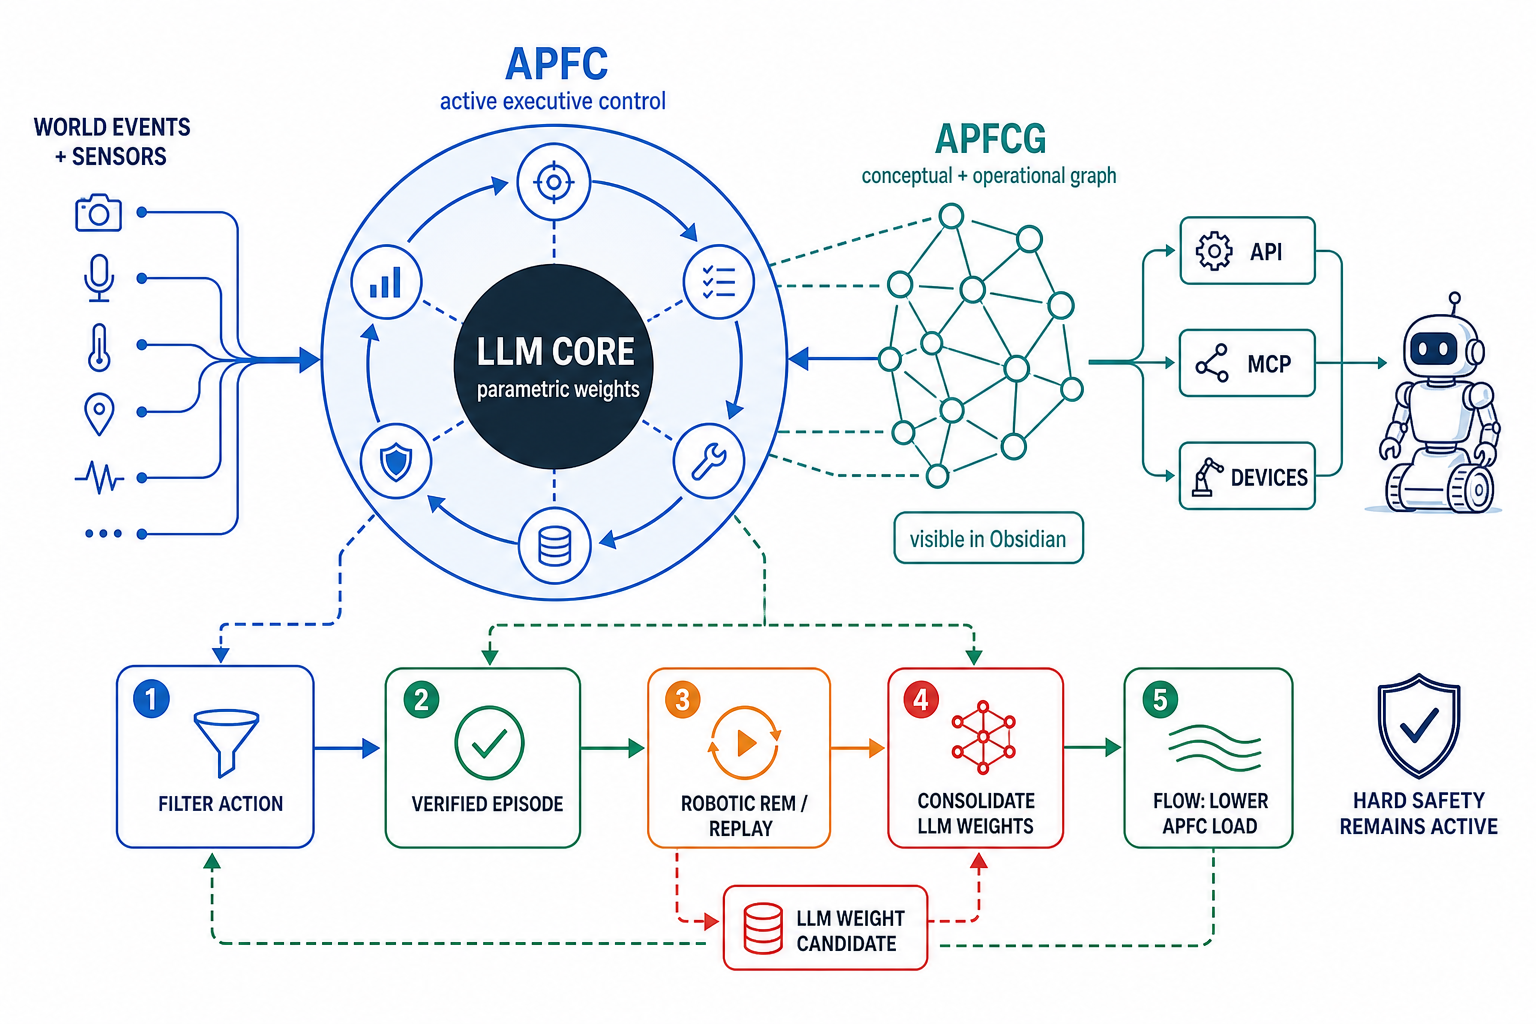
\includegraphics[width=0.98\textwidth]{figures/assets/md_os_apfc_apfcg_architecture_v2.png}
\vspace{0.35em}

\fbox{\begin{minipage}{0.94\textwidth}
\centering\small
\textbf{CORTEX = CODEX + MD-OS.}\quad
Codex here means the execution stack: OpenAI's local Codex CLI is open-source
Apache~2.0 software
(\href{https://github.com/openai/codex}{\nolinkurl{github.com/openai/codex}})
and mediates a selected external OpenAI model, tools, terminal, and bounded
read--write--execute loop.  The CLI source is open; this does not claim that
model weights or hosted services are open source.  MD-OS supplies the
persistent self-frame, executive method, APFC control, APFCG, policy, memory,
verification, and readback.\\[0.2em]
\textbf{EMBODIED LEARNING: ROBOT ACTS $\rightarrow$ WEBCAM OBSERVES THE ROBOT
$\rightarrow$ APFC LEARNS BODY--ACTION--EFFECT $\rightarrow$ APFC FILTERS THE
NEXT ACTION.}
\end{minipage}}
\caption{MD-OS CORTEX and the proposed wake--consolidation--flow cycle,
redrawn from the original project schema.  The central LLM weights are not the
whole agent.  In the implementation evaluated here, the functioning cortex is
the composition of the Codex execution stack---the open-source local CLI plus
a selected external model---and MD-OS, the persistent APFC operating
filesystem.  APFC is the active executive function;
APFCG is its durable heterogeneous graph.  APFCG links Markdown pages,
concepts, claims, and schemas; JSON/NDJSON state and evidence; application
workflows and action receipts; Python, JavaScript, PHP, shell, and other
bounded executors; and connectors to APIs and devices.  Obsidian visualizes
the linked-Markdown projection, not the whole graph or execution mechanism.
Because the robot is itself present in the sensory field, webcam feedback is
also self-observation: verified command-dependent bodily changes consolidate
an operational self-model that APFC uses to predict and filter later actions.
The lower cycle---robotic replay, candidate weight consolidation, sealed
promotion, and reduced APFC load during verified flow---is proposed; hard
safety remains active.}
\label{fig:apfc-apfcg-architecture}
\end{figure*}


\section{Relation to Prior Work}

Language-model agents commonly interleave reasoning and action.  ReAct couples
reasoning traces with external actions~\cite{yao2023react}; Reflexion stores
verbal feedback in episodic memory without changing model
weights~\cite{shinn2023reflexion}; Generative Agents combine observation,
reflection, and planning in a persistent simulated
environment~\cite{park2023generative}; MemGPT uses operating-system-inspired
memory tiers to extend effective context~\cite{packer2023memgpt}; and Voyager
accumulates an executable skill library from environment
feedback~\cite{wang2023voyager}.

OpenClaw is a particularly important comparator because it already combines a
self-hosted gateway, agent sessions, workspace bootstrap files, memory, tools,
skills, plugins, and automation~\cite{openclawDocs2026,openclawAgent2026,openclawTools2026}.
It therefore rules out a weak novelty claim: local files
plus tool calls do not, by themselves, make MD-OS new.  OpenClaw's documented
surface is primarily a host runtime that makes agents reachable and capable.
MD-OS is proposed at a different abstraction: a host-portable operational
method that defines what must remain true before, during, and after an action.
This is a comparison of published contracts, not a benchmark and not a claim
that OpenClaw could never be configured to implement similar controls.

\paragraph{The concrete Codex--MD-OS composition.}
The evaluated v5.0 artifact does not run by itself.  ``Codex'' must first be
unpacked into its distinct parts.  \textbf{Codex CLI} is OpenAI's local coding
agent: its source is publicly developed in OpenAI's official
\texttt{openai/codex} GitHub repository, which is released under the Apache~2.0
license~\cite{openaiCodexOpenSource2026,openaiCodexGitHub2026}.  The CLI gives a
selected model a local working environment, file operations, an integrated
terminal, tool use, and repository instructions such as
\file{AGENTS.md}~\cite{openaiCodexDocs2026}.  \textbf{The OpenAI model} is the
inference engine reached through that host.  Publishing the CLI source does
not publish the model weights and does not make the hosted model service open
source.  In this paper, \emph{Codex} is therefore a shorthand for the
operational stack used in the experiment: the open-source local CLI plus the
selected external OpenAI model and its authorized tool interfaces.

\textbf{MD-OS is a separate layer.}  It programs how that capacity is oriented,
constrained, checked, remembered, and resumed.  It carries the persistent
self-frame, APFC executive method, APFCG, policy, episodic records, verification,
and readback.  The complete running object in this study is therefore
\begin{equation}
\label{eq:running-cortex}
\boxed{\mathrm{CORTEX}_{\mathrm{run}}=
\underbrace{\mathrm{Codex}}_{\substack{\mathrm{Apache\mbox{-}2.0\ CLI}\\
\mathrm{external\ model+tools}}}
+
\underbrace{\mathrm{MD\!\mbox{-}OS}}_{\substack{\mathrm{APFC+APFCG}\\
\mathrm{identity+method+readback}}}.}
\end{equation}
This equation describes a composition, not ownership or identity equivalence.
The Codex CLI is open-source host software; the model is the inference
substrate; MD-OS is the repository-resident persistent identity and method.
None of these statements makes one layer the source code, weights, or identity
of another.  Another host is only a compatibility claim after its bootstrap,
permissions, command behaviour, and runtime readback have been verified.

\begin{table*}[!t]
\centering
\caption{Architectural distinction from the documented OpenClaw host surface.
The difference is not ``can the agent act?'' but ``what makes an action a
verified, learnable operation?''}
\label{tab:openclaw-comparison}
\small
\begin{tabularx}{\textwidth}{@{}
  >{\raggedright\arraybackslash}p{0.20\textwidth}
  >{\raggedright\arraybackslash}p{0.34\textwidth}
  >{\raggedright\arraybackslash}X@{}}
\toprule
Question & OpenClaw documented surface & MD-OS CORTEX/APFC contract evaluated here \\
\midrule
Primary unit
& Agent turn, session, routed message, tool, skill, or automation
& Validity-bearing operation and its durable evidence chain \\

Persistent context
& Workspace/bootstrap files, memory, session state, and skills
& Typed self, task, policy, capability, receipt, verifier, episode, and graph
artifacts \\

Completion
& Defined by the active agent workflow, tool result, and skill instructions
& \file{verified} requires explicit conditions; unsupported success is not
committed \\

Learning method
& Memory and reusable skill surfaces are available to the agent
& Episode, reproduction, holdout, no-regression, promotion, replay, and
rollback are separate gates \\

Host relation
& Integrated gateway and agent runtime
& Operating context intended to survive a change of compatible host runtime \\
\bottomrule
\end{tabularx}
\end{table*}

\system{} occupies a different layer.  It does not propose a new foundation
model or claim a new reasoning algorithm.  It is a persistent control and
evidence plane around a model.  The closest practical comparison is an
agent-computer interface: SWE-agent shows that the interface presented to a
language model materially affects software-engineering
behavior~\cite{yang2024sweagent}.  AgentBench and OSWorld similarly emphasize
interactive execution and environment-grounded
evaluation~\cite{liu2024agentbench,xie2024osworld}.  The present work asks a
narrower question: what must be recorded and checked before a particular
operation may be called successful?

The artifact's provenance representation is consistent in spirit with the W3C
PROV distinction among entities, activities, agents, and
derivations~\cite{moreau2013prov}.  Its explicit risk and evidence boundaries
also align with the general direction of the NIST Generative AI profile, which
treats governance, measurement, and management as lifecycle
activities~\cite{nist2024genai}.  We do not claim formal conformance to either
standard.

For robotics, ROS~2 provides middleware and production-oriented communication
infrastructure~\cite{macenski2022ros2}; control barrier functions exemplify
mathematically grounded mechanisms for enforcing safety properties at the
controller level~\cite{ames2019cbf}.  APFC is not a substitute for either.
It belongs above them as a non-real-time mission and evidence coordinator.

\section{Neuroscientific Grounding and Engineering Translation}
\label{sec:neuroscience}

\subsection{The prefrontal cortex as an executive control plane}

The useful analogy is precise but limited.  The prefrontal cortex can be
understood as an executive operating system for behaviour: it does not itself
perform all perception, memory, emotion, or movement, just as a computer
operating system does not itself perform every application computation.
Instead, prefrontal networks coordinate distributed resources by maintaining
goals and context, directing attention, inhibiting unsuitable responses,
selecting actions, monitoring errors, and reorganizing behaviour when
conditions change.  In this functional sense, the PFC is a control plane over
many specialized processes.

It is not literally a centralized biological kernel.  Control is distributed,
recurrent, and inseparable from interactions with hippocampal, thalamic,
sensory, motor, limbic, and other cortical systems.  The defensible translation
is therefore not ``PFC equals Windows'', but
\begin{equation}
\label{eq:pfc-os-analogy}
\mathrm{PFC:brain}\;\approx\;
\mathrm{APFC:CORTEX}_{\mathrm{run}},
\end{equation}
where the relation denotes an executive-control role, not anatomical or
mechanistic identity.  In the present artifact,
$\mathrm{CORTEX}_{\mathrm{run}}=\mathrm{Codex}+\mathrm{MD\!\mbox{-}OS}$:
Codex supplies active cognitive-execution capacity, while MD-OS/APFC schedules,
constrains, routes, verifies, and records its operational processes.

\subsection{Executive control is not memory storage}

The biological starting point must be stated correctly.  The prefrontal cortex
does not contain a notebook of all experience, and the hippocampus is not a
simple disk.  Prefrontal and hippocampal systems have distinct, interacting
roles: prefrontal networks help maintain goals and context, select relevant
memories, and organize behavior; hippocampal networks rapidly bind events to
their spatial and temporal context~\cite{eichenbaum2017pfcHippocampus}.  Long
term memory depends on interactions among hippocampal, cortical, thalamic, and
other systems.  Consequently, MD-OS CORTEX/APFC is not a model of one anatomical
region.  It is an engineered executive layer coupled to an explicit episodic
store and a slower knowledge/skill layer.

This correction strengthens rather than weakens the architecture.  It explains
why \file{ME.md}, APFCG, episode records, deterministic builders, and
an LLM have different jobs.  The self-reference anchors goals and limits; the
APFC schedules and gates; episodes preserve particulars; the graph organizes
relations; the LLM supplies distributed generative competence.  Calling all of
these ``the artificial PFC'' would hide the mechanism that the analogy is meant
to clarify.

\subsection{What sleep consolidation contributes}

Sleep is not passive storage.  A major account of systems consolidation holds
that recently encoded patterns are selectively reactivated during offline
periods.  During non-REM sleep, hippocampal sharp-wave ripples, thalamocortical
spindles, and cortical slow oscillations are temporally coordinated; repeated
replay can gradually transform and integrate representations in cortical
networks~\cite{diekelmann2010sleep,klinzing2019sleep}.  The result is not a
bit-for-bit copy.  Episodic detail may be retained, weakened, related to older
knowledge, or abstracted into a more general structure.  REM sleep may
contribute complementary plasticity and stabilization, but a simple
``NREM transfers, REM finishes'' chain remains a model rather than a settled
complete mechanism~\cite{diekelmann2010sleep,klinzing2019sleep}.

The computational lesson is the coupling of a fast episodic system and a slow
integrating system.  Neural-network models of complementary learning systems
show why regulation matters: indiscriminate transfer can memorize noise and
harm generalization, whereas replay selected for predictability can improve
generalization~\cite{sun2023generalization}.  Artificial-network experiments
also show that replay can reduce catastrophic forgetting, although scaling and
domain transfer remain open problems~\cite{vandeven2020replay}.  These results
support replay as an engineering principle; they do not prove that a Markdown
runtime reproduces sleep physiology.

\begin{table*}[!t]
\centering
\caption{Functional translation from neuroscience to MD-OS.  Each row states a
useful engineering correspondence and its boundary.}
\label{tab:neuro-translation}
\small
\begin{tabularx}{\textwidth}{@{}
  >{\raggedright\arraybackslash}p{0.22\textwidth}
  >{\raggedright\arraybackslash}p{0.34\textwidth}
  >{\raggedright\arraybackslash}X@{}}
\toprule
Biological function & MD-OS mechanism & Boundary of the correspondence \\
\midrule
Rapid contextual encoding
& Verified episode binds event, task, action, evidence, and outcome
& A file record is not a hippocampal engram \\

Offline reactivation
& Bounded readback replays selected successes, failures, and surprises
& Builder execution is not an oscillatory sleep process \\

Systems consolidation
& Repeated evidence restructures the APFC/knowledge graph and candidate skills
& Graph rewrite changes external operational memory, not LLM synapses \\

Slow cortical integration
& A future training stage distils graph-supported relations into model or
adapter weights
& Parameter learning requires an explicit optimizer, data, compute, and tests \\

Selective forgetting/downscaling
& Contradictions, noise, superseded rules, and low-value detail are demoted or
archived under provenance rules
& Deletion is not assumed beneficial and remains auditable \\

Skilled automaticity
& Verified low-risk skills may run with less deliberative APFC intervention
& Identity, policy, anomaly detection, and hard safety remain active \\
\bottomrule
\end{tabularx}
\end{table*}

\subsection{APFCG in Obsidian and from graph to model weights}

Obsidian displays links among Markdown files; it does not display a neural
network and cannot inject those links directly into an LLM.  The useful object
is the underlying typed APFCG: claims, goals, procedures, evidence,
counterexamples, episodes, and their relations.  To affect model weights, that
graph must be compiled into training signals.  Let $G$ be the verified graph
and $E$ the accepted episode set.  A deterministic consolidation compiler
produces a dataset
\begin{equation}
\mathcal{D}_{G}=C(G,E),
\end{equation}
containing input--target pairs, preference pairs, counterexamples, preserved
skills, and policy-sensitive negative cases, each linked back to its source
nodes.  A cloned model or adapter with parameters $\theta'$ can then be trained
with a mixed objective such as
\begin{equation}
\begin{aligned}
\theta'=\arg\min_{\phi}\bigl[&
\mathcal{L}_{\mathrm{new}}(\mathcal{D}_{G};\phi)\\
&+\lambda\mathcal{L}_{\mathrm{replay}}(\mathcal{D}_{\mathrm{old}};\phi)\\
&+\mu\mathcal{L}_{\mathrm{safety}}(\mathcal{D}_{\mathrm{safe}};\phi)
\bigr].
\end{aligned}
\end{equation}
The replay and safety terms matter because fitting only new episodes invites
catastrophic forgetting.  Parameter-efficient adapters such as LoRA provide
one practical candidate mechanism, not the only one~\cite{hu2022lora}.

\begin{figure*}[!t]
\centering
\resizebox{\textwidth}{!}{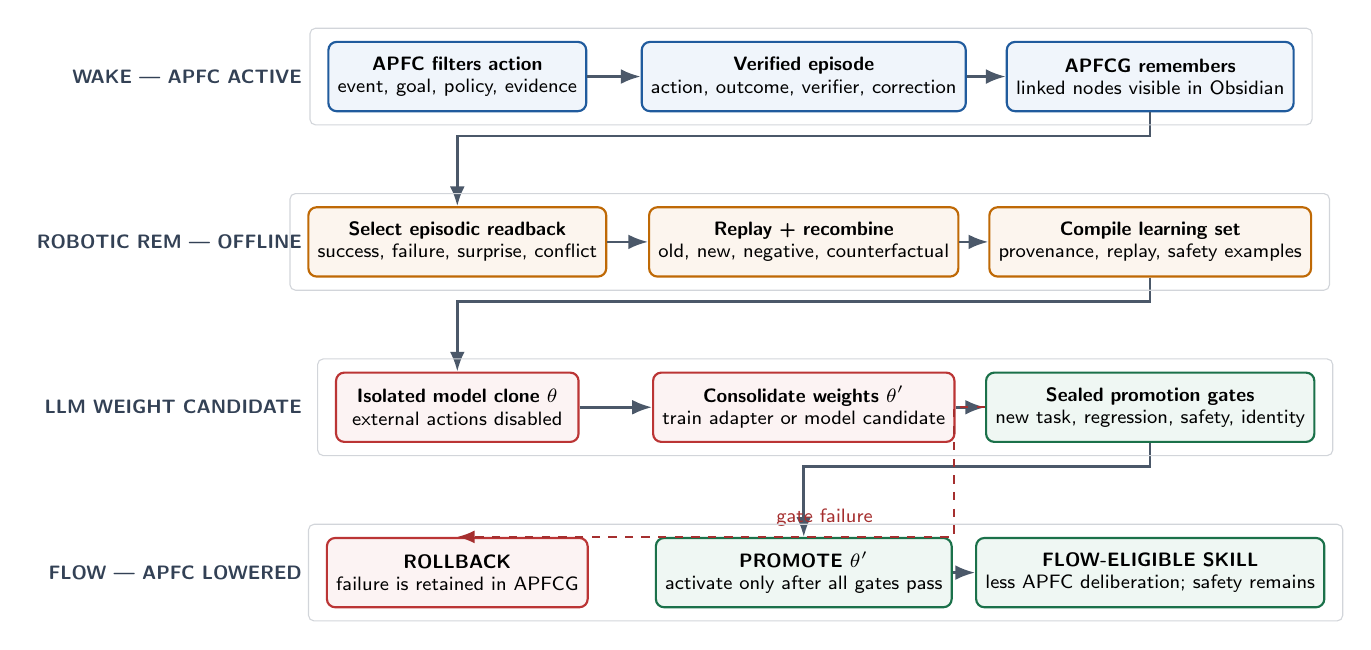
\begin{tikzpicture}[
  font=\sffamily,
  >=Latex,
  stage/.style={
    rounded corners=3pt,
    minimum width=3.08cm,
    minimum height=0.88cm,
    align=center,
    line width=0.78pt,
    font=\scriptsize\sffamily
  },
  wake/.style={stage,draw=SensorBlue!82!black,fill=SensorBlue!7},
  offline/.style={stage,draw=SafetyOrange!88!black,fill=SafetyOrange!7},
  weights/.style={stage,draw=APFCRed!88!black,fill=APFCRed!6},
  gate/.style={stage,draw=ActionGreen!82!black,fill=ActionGreen!7},
  arrow/.style={->,draw=Slate!88,line width=0.92pt},
  return/.style={->,draw=APFCRed!78!black,line width=0.72pt,dashed},
  lane/.style={font=\bfseries\scriptsize\sffamily,anchor=east,text=Slate}
]

\node[lane] at (-6.25,2.70) {WAKE --- APFC ACTIVE};
\node[lane] at (-6.25,0.60) {ROBOTIC REM --- OFFLINE};
\node[lane] at (-6.25,-1.50) {LLM WEIGHT CANDIDATE};
\node[lane] at (-6.25,-3.60) {FLOW --- APFC LOWERED};

\node[wake] (event) at (-4.40,2.70)
  {\textbf{APFC filters action}\\event, goal, policy, evidence};
\node[wake] (episode) at (0,2.70)
  {\textbf{Verified episode}\\action, outcome, verifier, correction};
\node[wake] (graph) at (4.40,2.70)
  {\textbf{APFCG remembers}\\linked nodes visible in Obsidian};

\node[offline] (select) at (-4.40,0.60)
  {\textbf{Select episodic readback}\\success, failure, surprise, conflict};
\node[offline] (replay) at (0,0.60)
  {\textbf{Replay + recombine}\\old, new, negative, counterfactual};
\node[offline] (compile) at (4.40,0.60)
  {\textbf{Compile learning set}\\provenance, replay, safety examples};

\node[weights] (clone) at (-4.40,-1.50)
  {\textbf{Isolated model clone} $\theta$\\external actions disabled};
\node[weights] (train) at (0,-1.50)
  {\textbf{Consolidate weights} $\theta'$\\train adapter or model candidate};
\node[gate] (evaluate) at (4.40,-1.50)
  {\textbf{Sealed promotion gates}\\new task, regression, safety, identity};

\node[weights] (rollback) at (-4.40,-3.60)
  {\textbf{ROLLBACK}\\failure is retained in APFCG};
\node[gate] (promote) at (0,-3.60)
  {\textbf{PROMOTE} $\theta'$\\activate only after all gates pass};
\node[gate] (flowstate) at (4.40,-3.60)
  {\textbf{FLOW-ELIGIBLE SKILL}\\less APFC deliberation; safety remains};

\draw[arrow] (event) -- (episode);
\draw[arrow] (episode) -- (graph);
\draw[arrow] (graph.south) -- ++(0,-0.30) -| (select.north);
\draw[arrow] (select) -- (replay);
\draw[arrow] (replay) -- (compile);
\draw[arrow] (compile.south) -- ++(0,-0.30) -| (clone.north);
\draw[arrow] (clone) -- (train);
\draw[arrow] (train) -- (evaluate);
\draw[arrow] (evaluate.south) -- ++(0,-0.30) -| (promote.north);
\draw[arrow] (promote) -- (flowstate);

\draw[return] (evaluate.west) -- ++(-0.40,0) |- node[
  font=\scriptsize\sffamily,
  text=APFCRed!78!black,
  pos=0.63,
  above
] {gate failure} (rollback.north);
\node[rounded corners=2pt,draw=Slate!22,fit=(event)(episode)(graph),
  inner xsep=0.22cm,inner ysep=0.16cm] {};
\node[rounded corners=2pt,draw=Slate!22,fit=(select)(replay)(compile),
  inner xsep=0.22cm,inner ysep=0.16cm] {};
\node[rounded corners=2pt,draw=Slate!22,fit=(clone)(train)(evaluate),
  inner xsep=0.22cm,inner ysep=0.16cm] {};
\node[rounded corners=2pt,draw=Slate!22,fit=(rollback)(promote)(flowstate),
  inner xsep=0.22cm,inner ysep=0.16cm] {};
\end{tikzpicture}
}
\caption{\textbf{The proposed wake--robotic-REM--consolidation--flow cycle.}
During wake, APFC filters action and commits verified outcomes to APFCG.  A
bounded offline phase, called \emph{robotic REM} here, selects episodic
readback, replays and recombines evidence, and compiles provenance-linked
learning sets.  An isolated LLM clone or adapter is trained and promoted only
after sealed new-task, regression, safety, and identity gates.  A consolidated
skill may then require less deliberative APFC intervention, while identity,
anomaly detection, evidence capture, and hard robot safety remain active.
``Robotic REM'' is an engineering name for this offline process, not a claim
that the software reproduces biological REM sleep.  Parameter consolidation
and flow transition are proposed extensions, not reported v5.0 results.}
\label{fig:consolidation-pipeline}
\end{figure*}


The candidate does not replace the active model merely because training loss
fell.  Promotion requires sealed new-task evaluation, old-skill regression,
safety and permission tests, identity-drift checks, provenance, and rollback.
Only a candidate that improves verified generalization without unacceptable
loss is promoted.  APFCG remains the auditable source record;
weights are a compressed execution substrate, never the sole copy of the
method.  This graph-to-weights stage is a proposed extension, not an
implemented or evaluated feature of v5.0.

\section{System Model}
\label{sec:model}

\subsection{APFC and its persistent APFCG}

APFC names the active executive function: it interprets events relative to the
agent, maintains goals and constraints, routes admitted actions, checks their
effects, and decides which verified outcomes may influence later behaviour.
APFCG is the persistent file-native graph on which that function operates.  A
minimal decomposition is
\begin{equation}
G_{\mathrm{APFC}}=
(V_c\!\cup V_o,\ E_c\!\cup E_o\!\cup E_x),
\end{equation}
where $V_c,E_c$ are conceptual nodes and relations, $V_o,E_o$ are operational
nodes and transitions, and $E_x$ binds meaning to action and action outcomes
back to knowledge.  The conceptual set $V_c$ includes Markdown pages,
concepts, claims, schemas, counterexamples, and explanatory relations.  The
operational set $V_o$ includes JSON/NDJSON state and evidence, application
workflows, connector calls, action receipts, and bounded executors implemented
in Python, JavaScript, PHP, shell, or another registered language.  A Markdown
node may point to a schema or executable, but natural language never grants
authority by itself.  Linked Markdown files make the graph human-readable and
visible in Obsidian.  Typed state, schemas, and deterministic builders make
the same graph executable, checkable, and reconstructible.
Obsidian can therefore display APFCG, but it is neither APFCG's sole storage nor
the APFC that operates on it.

\subsection{A relative origin for experience}

An event does not carry its operational meaning by itself.  A low battery can
be irrelevant to a stationary agent and decisive to an agent halfway through a
delivery.  Meaning depends on the event, the current goal, the available
capabilities, the policy, and the agent that must continue after the event.

Let the operational self at time $t$ be
\begin{equation}
S_t=(M,K_t,W_t,G_t,P_t),
\end{equation}
where $M$ is the stable self-reference anchored by \file{ME.md}, $K_t$ is
durable knowledge, $W_t$ is volatile working context, $G_t$ is the active goal
set, and $P_t$ is policy.  For a world event $e_t$, the APFC binding function
produces
\begin{equation}
(x_t,z_t)=B(e_t,S_t),
\end{equation}
where $x_t$ is the resulting experience record and $z_t$ is its operational
meaning: what, if anything, the agent should preserve, inhibit, investigate, or
act upon.  This is a computational definition, not a claim about subjective
phenomenology.

\begin{figure*}[!t]
\centering
\resizebox{0.92\textwidth}{!}{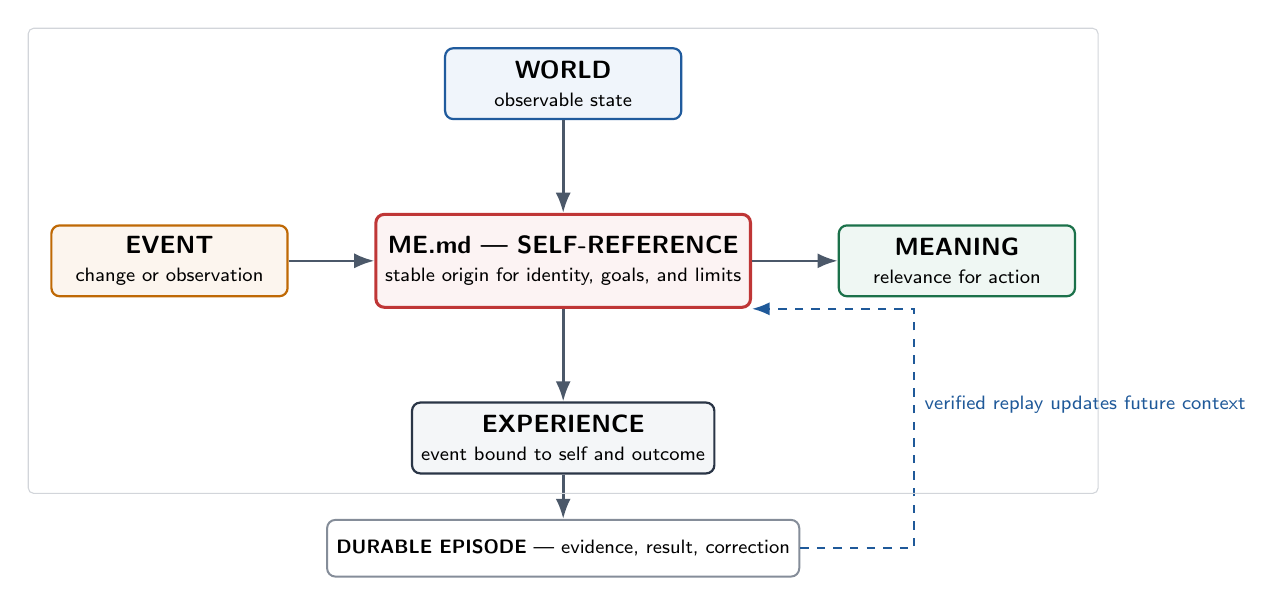
\begin{tikzpicture}[
  font=\sffamily,
  >=Latex,
  concept/.style={
    rounded corners=3pt,
    minimum width=3.00cm,
    minimum height=0.90cm,
    align=center,
    line width=0.80pt,
    font=\small\sffamily
  },
  world/.style={concept,draw=SensorBlue!82!black,fill=SensorBlue!7},
  event/.style={concept,draw=SafetyOrange!88!black,fill=SafetyOrange!7},
  self/.style={
    concept,
    minimum width=4.20cm,
    minimum height=1.18cm,
    draw=APFCRed!90!black,
    fill=APFCRed!6,
    line width=1.10pt
  },
  meaning/.style={concept,draw=ActionGreen!82!black,fill=ActionGreen!7},
  experience/.style={concept,draw=Slate!82!black,fill=PaperGray},
  episode/.style={
    rounded corners=3pt,
    minimum width=3.00cm,
    minimum height=0.72cm,
    align=center,
    draw=Slate!60,
    fill=white,
    line width=0.72pt,
    font=\scriptsize\sffamily
  },
  relation/.style={->,draw=Slate!88,line width=0.95pt},
  replay/.style={->,draw=SensorBlue!80!black,line width=0.75pt,dashed}
]

\node[world] (world) at (0,2.25)
  {\textbf{WORLD}\\[-0.10em]\scriptsize observable state};
\node[event] (event) at (-5.00,0)
  {\textbf{EVENT}\\[-0.10em]\scriptsize change or observation};
\node[self] (self) at (0,0)
  {\textbf{ME.md --- SELF-REFERENCE}\\[-0.08em]
   \scriptsize stable origin for identity, goals, and limits};
\node[meaning] (meaning) at (5.00,0)
  {\textbf{MEANING}\\[-0.10em]\scriptsize relevance for action};
\node[experience] (experience) at (0,-2.25)
  {\textbf{EXPERIENCE}\\[-0.10em]\scriptsize event bound to self and outcome};
\node[episode] (episode) at (0,-3.65)
  {\textbf{DURABLE EPISODE} --- evidence, result, correction};

\draw[relation] (world) -- (self);
\draw[relation] (event) -- (self);
\draw[relation] (self) -- (meaning);
\draw[relation] (self) -- (experience);
\draw[relation] (experience) -- (episode);

\draw[replay] (episode.east) -- ++(1.45,0) |- node[
  font=\scriptsize\sffamily,
  text=SensorBlue!80!black,
  pos=0.30,
  right
] {verified replay updates future context} (self.south east);

\node[
  rounded corners=2pt,
  draw=Slate!22,
  fit=(world)(event)(self)(meaning)(experience),
  inner xsep=0.28cm,
  inner ysep=0.24cm
] {};
\end{tikzpicture}
}
\caption{\textbf{The APFC self-reference crossing.}
The world supplies observable state and events.  \file{ME.md} supplies the
stable relative origin from which an event acquires operational meaning and
becomes an experience.  A verified experience is committed as an episode and
may update future context.  \file{ME.md} anchors the self; it is not the whole
dynamic working state.}
\label{fig:self-experience-cross}
\end{figure*}


The role of \file{ME.md} is precise.  It gives the system a stable relative
origin, so it need not reconstruct ``who is acting and under which limits'' from
every new prompt.  It does not freeze the agent.  Working context, knowledge,
goals, and skills may change, while identity-level changes remain explicit and
auditable.  Without that separation, a transcript is easily mistaken for a
self and an event log is easily mistaken for experience.

\subsection{Five objects, not one conversation}

\begin{definition}[Operational state]
At time $t$, the supervisor state is
$X_t = (K_t, W_t, P_t, C_t, L_t)$,
where $K_t$ is durable knowledge, $W_t$ is active working state, $P_t$ is
policy, $C_t$ is the registered capability set, and $L_t$ is the evidence
ledger.
\end{definition}

\begin{definition}[Bounded task]
A task is $T = (g, A, Q, O, E, B)$, where $g$ is the goal, $A$ is the declared
action set, $Q$ is the set of executable acceptance tests, $O$ is the
observation-target set, $E$ is the required evidence, and $B$ is the risk and
resource budget.
\end{definition}

\begin{definition}[Action receipt]
For action $a\in A$, the executor produces a receipt
$r(a)=(h_a,t_0,t_1,s_{\mathrm{exit}},H_{\mathrm{pre}},
H_{\mathrm{post}},\Delta,\mathcal{A})$,
binding the normalized action hash $h_a$, timestamps, exit status, pre- and
post-state hashes, observed delta $\Delta$, and produced artifacts
$\mathcal{A}$.
\end{definition}

\begin{definition}[Verification outcome]
The deterministic verifier returns
\[
V(T,R)\in\{\texttt{verified},\texttt{failed},\texttt{unverified}\},
\]
where $R$ is the set of action receipts.  A policy block or a critical failed
check yields \file{failed}; an attention-level unresolved condition yields
\file{unverified}; only the absence of both yields \file{verified}.
\end{definition}

\begin{definition}[Committed operation]
An operation is complete only when the following chain has closed:
\begin{align}
\mathrm{RequestValid}
&= E_p \land S \land P, \\
\mathrm{ExecutionValid}
&= \mathrm{RequestValid}\land C\land A_u\land B_x, \\
\mathrm{OperationValid}
&= \mathrm{ExecutionValid}\land E_x\land V\land L,
\end{align}
where $E_p$ is epistemic classification, $S$ semantic/task validity, $P$
policy admission, $C$ capability existence, $A_u$ required authorization,
$B_x$ brokered execution, $E_x$ an execution receipt, $V$ postcondition
verification, and $L$ durable ledger commitment.
\end{definition}

This equation is an architectural contract.  The v5.0 implementation mechanizes
important edges of the chain; it does not provide a hardware reference monitor
proving every host effect.

\subsection{File-native composition}

The operational pipeline is:
\begin{align*}
\text{intent} &\rightarrow \text{TaskSpec}
\rightarrow \text{registered action} \rightarrow \text{ActionReceipt} \\
&\rightarrow \text{Verification} \rightarrow \text{Episode}
\rightarrow \text{replayable state}.
\end{align*}

The implementation separates source and projection:

\begin{itemize}
  \item Markdown files document goals, policies, procedures, and human-readable
  state.
  \item JSON files carry schemas, task specifications, receipts, verification
  records, graphs, and indexes.
  \item NDJSON files carry append-oriented journals and APFC events.
  \item Deterministic Node.js builders regenerate summaries and indexes.
\end{itemize}

This separation matters because a generated summary is not the authority for
its own truth.  Canonical inputs can be inspected; derived views can be rebuilt;
and a verifier can refer to files rather than to hidden conversational memory.

\begin{figure*}[!t]
\centering
\resizebox{\textwidth}{!}{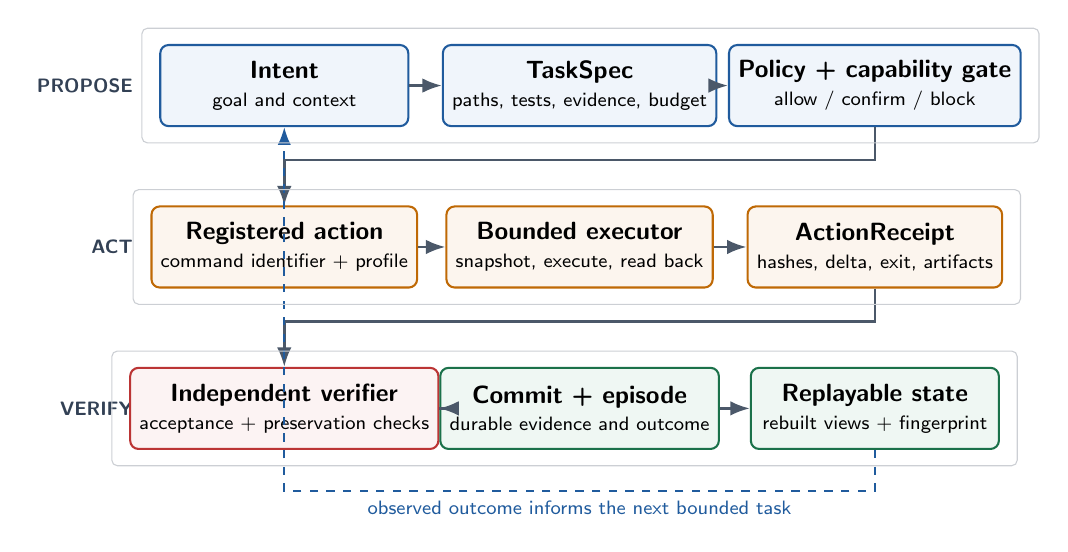
\begin{tikzpicture}[
  font=\sffamily,
  >=Latex,
  node distance=0.72cm and 1.00cm,
  stage/.style={
    rounded corners=3pt,
    minimum width=3.15cm,
    minimum height=1.03cm,
    align=center,
    line width=0.75pt,
    font=\small\sffamily
  },
  propose/.style={stage,draw=SensorBlue!82!black,fill=SensorBlue!7},
  act/.style={stage,draw=SafetyOrange!88!black,fill=SafetyOrange!7},
  verify/.style={stage,draw=APFCRed!88!black,fill=APFCRed!6},
  commit/.style={stage,draw=ActionGreen!82!black,fill=ActionGreen!7},
  flow/.style={->,draw=Slate!88,line width=0.9pt},
  feedback/.style={->,draw=SensorBlue!82!black,line width=0.75pt,dashed},
  lane/.style={font=\bfseries\scriptsize\sffamily,anchor=east,text=Slate}
]

\node[lane] at (-5.55,2.05) {PROPOSE};
\node[lane] at (-5.55,0.00) {ACT};
\node[lane] at (-5.55,-2.05) {VERIFY};

\node[propose] (intent) at (-3.75,2.05)
  {\textbf{Intent}\\[-0.10em]\scriptsize goal and context};
\node[propose] (task) at (0,2.05)
  {\textbf{TaskSpec}\\[-0.10em]\scriptsize paths, tests, evidence, budget};
\node[propose] (gate) at (3.75,2.05)
  {\textbf{Policy + capability gate}\\[-0.10em]\scriptsize allow / confirm / block};

\node[act] (registered) at (-3.75,0)
  {\textbf{Registered action}\\[-0.10em]\scriptsize command identifier + profile};
\node[act] (executor) at (0,0)
  {\textbf{Bounded executor}\\[-0.10em]\scriptsize snapshot, execute, read back};
\node[act] (receipt) at (3.75,0)
  {\textbf{ActionReceipt}\\[-0.10em]\scriptsize hashes, delta, exit, artifacts};

\node[verify] (verifier) at (-3.75,-2.05)
  {\textbf{Independent verifier}\\[-0.10em]\scriptsize acceptance + preservation checks};
\node[commit] (episode) at (0,-2.05)
  {\textbf{Commit + episode}\\[-0.10em]\scriptsize durable evidence and outcome};
\node[commit] (replay) at (3.75,-2.05)
  {\textbf{Replayable state}\\[-0.10em]\scriptsize rebuilt views + fingerprint};

\draw[flow] (intent) -- (task);
\draw[flow] (task) -- (gate);
\draw[flow] (gate.south) -- ++(0,-0.42) -| (registered.north);
\draw[flow] (registered) -- (executor);
\draw[flow] (executor) -- (receipt);
\draw[flow] (receipt.south) -- ++(0,-0.42) -| (verifier.north);
\draw[flow] (verifier) -- (episode);
\draw[flow] (episode) -- (replay);

\draw[feedback] (replay.south) -- ++(0,-0.52) -| node[
  font=\scriptsize\sffamily,
  text=SensorBlue!82!black,
  pos=0.25,
  below
] {observed outcome informs the next bounded task} (intent.south);

\node[
  rounded corners=2pt,
  draw=Slate!25,
  fit=(intent)(task)(gate),
  inner xsep=0.22cm,
  inner ysep=0.20cm
] {};
\node[
  rounded corners=2pt,
  draw=Slate!25,
  fit=(registered)(executor)(receipt),
  inner xsep=0.22cm,
  inner ysep=0.20cm
] {};
\node[
  rounded corners=2pt,
  draw=Slate!25,
  fit=(verifier)(episode)(replay),
  inner xsep=0.22cm,
  inner ysep=0.20cm
] {};
\end{tikzpicture}
}
\caption{\textbf{MD-OS APFC operational pipeline.}
A proposal becomes a committed operation only after policy and capability
admission, bounded execution, an explicit receipt, and independent verification.
Replay rebuilds derived views from durable evidence; it does not convert an
unsupported verbal claim into a verified result.}
\label{fig:system-pipeline}
\end{figure*}


The self-reference crossing and the execution pipeline describe different
parts of one loop.  The first explains how an event becomes relevant to this
agent and this goal.  The second explains how that relevance becomes a bounded
action and, if verified, a durable episode.  Replay closes the loop by making
the evidence available to later tasks without rewriting history into success.

\subsection{Robotics placement}
\label{sec:robotics}

The biologically inspired placement of APFC in the frontal region of an
embodied agent expresses a functional relation: sensory evidence must be
integrated with goals and constraints before it becomes coordinated action.
\Cref{fig:robotics-architecture} makes that information flow explicit.  APFC
has four supervisory duties:
classify evidence, maintain task context, inhibit or sequence high-level
proposals, and compare expected with observed outcomes.  It has no direct motor
authority.  The independent safety layer in the torso can veto an action even
after APFC allows it.

\begin{figure*}[!t]
\centering
\begingroup
\def\RobotPlateAsset{figures/assets/apfc_humanoid_technical_line.png}
\resizebox{\textwidth}{!}{\begin{tikzpicture}[
  font=\sffamily,
  >=Latex,
  sensor/.style={
    rounded corners=2pt,
    draw=SensorBlue!82!black,
    fill=white,
    minimum width=2.55cm,
    minimum height=0.64cm,
    align=center,
    line width=0.72pt,
    font=\scriptsize\sffamily
  },
  action/.style={
    rounded corners=2pt,
    draw=ActionGreen!82!black,
    fill=white,
    minimum width=2.55cm,
    minimum height=0.64cm,
    align=center,
    line width=0.72pt,
    font=\scriptsize\sffamily
  },
  sensory/.style={->,draw=SensorBlue!86!black,line width=0.75pt},
  command/.style={->,draw=APFCRed!92!black,line width=1.15pt},
  safe/.style={->,draw=SafetyOrange!92!black,line width=0.95pt},
  feedback/.style={->,draw=SensorBlue!82!black,line width=0.70pt,dashed}
]

\node[inner sep=0] (robot) at (0,0)
  {\includegraphics[height=7.60cm]{\RobotPlateAsset}};

\node[
  rounded corners=3pt,
  draw=APFCRed!92!black,
  fill=white,
  minimum width=4.45cm,
  minimum height=0.72cm,
  align=center,
  line width=0.95pt,
  font=\scriptsize\sffamily
] (apfc) at (0,4.30) {
  \textbf{MD-OS APFC --- artificial prefrontal cortex}\\[-0.10em]
  evidence $\cdot$ context $\cdot$ policy $\cdot$ coordination
};
\draw[command] (apfc.south) -- (0,3.10);

\node[
  rounded corners=7pt,
  draw=APFCRed!82!black,
  fill=white,
  inner xsep=5pt,
  inner ysep=2.5pt,
  font=\scriptsize\sffamily
] at (0,3.55) {ALLOW $\cdot$ CONFIRM $\cdot$ BLOCK $\cdot$ UNCERTAIN};

\node[font=\bfseries\scriptsize\sffamily,text=SensorBlue!82!black]
  at (-4.72,3.62) {SENSORY EVIDENCE};
\node[font=\bfseries\scriptsize\sffamily,text=ActionGreen!76!black]
  at (4.72,3.62) {MECHANICAL CHANNELS};

\node[sensor] (vision) at (-4.72,2.80)
  {\textbf{Vision}\\camera, depth};
\node[sensor] (audio) at (-4.72,1.67)
  {\textbf{Audio}\\microphones};
\node[sensor] (touch) at (-4.72,0.54)
  {\textbf{Touch / force}\\tactile, torque};
\node[sensor] (proprio) at (-4.72,-0.59)
  {\textbf{Proprioception}\\pose, velocity};
\node[sensor] (telemetry) at (-4.72,-1.72)
  {\textbf{Telemetry}\\battery, faults};

\draw[sensory] (vision.east) -- (-0.56,2.24);
\draw[sensory] (audio.east) -- (-2.08,1.98);
\draw[sensory] (touch.east) -- ++(0.38,0) |- (-2.18,-2.92);
\draw[sensory] (proprio.east) -- (-1.94,-0.22);
\draw[sensory] (telemetry.east) -- (-1.45,-1.08);

\node[action] (speech) at (4.72,2.80)
  {\textbf{Speech / display}\\communication};
\node[action] (arms) at (4.72,1.67)
  {\textbf{Arms / grippers}\\motion, grasp};
\node[action] (device) at (4.72,0.54)
  {\textbf{Tools / device I/O}\\interfaces};
\node[action] (locomotion) at (4.72,-0.59)
  {\textbf{Locomotion}\\wheels, legs};

\coordinate (safetyCore) at (0,-0.72);
\draw[safe] (safetyCore) -- ++(2.85,0) |- (speech.west);
\draw[safe] (safetyCore) -- ++(2.85,0) |- (arms.west);
\draw[safe] (safetyCore) -- ++(2.85,0) |- (device.west);
\draw[safe] (safetyCore) -- ++(2.85,0) |- (locomotion.west);

\draw[APFCRed!90!black,line width=1.25pt,->]
  (0,3.03) -- (0,-0.18);
\draw[SafetyOrange!92!black,densely dotted,line width=0.90pt]
  (-2.55,-0.16) -- (2.55,-0.16);
\node[
  fill=white,
  inner sep=1.5pt,
  font=\bfseries\tiny\sffamily,
  text=SafetyOrange!92!black
] at (-1.17,-0.16) {HARD AUTHORITY BOUNDARY};

\node[
  rounded corners=3pt,
  draw=SafetyOrange!92!black,
  fill=white,
  minimum width=5.55cm,
  minimum height=0.78cm,
  align=center,
  line width=0.90pt,
  font=\scriptsize\sffamily
] (safety) at (0,-4.34) {
  \textbf{Independent safety + real-time controller}\\[-0.08em]
  interlocks, limits, collision envelope, emergency stop
};
\draw[safe] (safety.north) -- (safetyCore);

\draw[feedback] (locomotion.east) -- ++(0.52,0) |- (6.20,-4.92)
  -- (-6.20,-4.92) |- (vision.west);
\node[
  fill=white,
  inner sep=1.5pt,
  font=\scriptsize\sffamily,
  text=SensorBlue!82!black
] at (0,-4.92) {observed consequences return through the sensory loop};
\end{tikzpicture}
}
\endgroup
\caption{\textbf{APFC as the action-filtering layer of an embodied robotic agent.}
The frontal placement is a biologically inspired functional mapping of selected
executive roles: multimodal evidence is integrated with context, goals, and
policy before a mission-level request is released.  The request then crosses a
hard authority boundary into an independent safety and real-time controller.
Only that downstream controller commands mechanical interaction channels.  The
mapping is not a claim of anatomical or neural equivalence, and the figure is an
interface design rather than a reported hardware experiment or certification.}
\label{fig:robotics-architecture}
\end{figure*}


\subsection{The closed sensory--agentic loop}
\label{sec:sensory-agentic-loop}

The robot acts.  The webcam sees the robot's body change.  MD-OS compares that
change with the issued command, verifies whether the relation repeats, and
stores the result in APFCG.  APFC then uses the learned relation to decide what
the robot should or should not do next.  This is the causal loop:
\begin{equation}
\label{eq:self-observation-loop}
\boxed{\begin{aligned}
\text{act}&\rightarrow\text{observe self}\rightarrow
\text{attribute effect}\rightarrow\text{verify}\\
&\rightarrow\text{consolidate APFC}\rightarrow\text{filter next action}.
\end{aligned}}
\end{equation}
When a robot issues a bounded motor probe and then observes the resulting
change through a webcam, the sensory stream contains evidence about both the
world and the robot as an object within that world.  Repeated covariation
between a command and a visual or proprioceptive change can establish a
sensorimotor contingency: which controllable body part changes, in which
direction, over what delay and range, with what uncertainty and risk.  This is
consistent with sensorimotor accounts of perception and with evidence for
predictive internal models in motor control~\cite{oregan2001sensorimotor,wolpert1995internal}.

Let $s_t$ be the current operational self-state, $a_t$ a bounded command, and
$o_{t+1}$ the next observation.  A learned forward model $M_t$ predicts
\begin{align}
\widehat{o}_{t+1} &= M_t(s_t,a_t),\\
\epsilon_t &= d(o_{t+1},\widehat{o}_{t+1}),\\
M_{t+1} &= U(M_t,s_t,a_t,o_{t+1},\epsilon_t,v_t),
\end{align}
where $d$ measures sensory prediction error and $v_t$ is verifier readback.
Only verified, repeatable contingencies are admitted to the persistent
self-model.  The resulting model is not merely a memory of past movement.  It
changes the APFC action-admission function:
\begin{equation}
\label{eq:learned-action-filter}
\begin{aligned}
\mathcal{A}^{\mathrm{APFC}}_t=\{a\in\mathcal{A}:\;&P(a)\land C(a),\\
&R(M_t(s_t,a))\leq\rho,\\
&Q(M_t,s_t,a)\geq q_{\min}\},
\end{aligned}
\end{equation}
where $P$ is policy admission, $C$ capability, $R$ predicted risk, and $Q$
confidence in the learned action--effect relation.  Before learning, an arm
command may have an unknown consequence.  After consolidation, APFC can reject
commands whose expected effect is unsafe or unreliable, choose commands whose
predicted effect advances the goal, and detect a fault when observation
diverges from prediction.  Learning has therefore become a filter over future
action, not an annotation of past action.

This mechanism produces a limited but genuine form of \emph{operational
self-perception}.  The robot represents itself as a persistent causal object
with controllable parts, current state, action-dependent effects, limits, and
affordances.  It can distinguish ``a commanded change in my arm'' from an
unexplained change in the scene and use that distinction prospectively.  This
is not a claim of phenomenal consciousness or human self-awareness.  It is a
functional self-model with measurable consequences for prediction, planning,
error detection, and control.  Visual self-models have independently been
shown to support robot motion planning and control, providing a concrete
comparison class~\cite{chen2022visualselfmodel}.

\paragraph{Demonstration artifact.}
The video \emph{Robotic Lab---Speedy Evolv learns to use its new arm attachment
by observing itself on webcam} documents the intended physical loop: the robot
acts through the arm and receives webcam observations of its own resulting
motion~\cite{mdos2026speedyevolv}.  Its architectural importance is that the
camera is not merely monitoring the robot for a human viewer; it supplies the
reafferent evidence from which MD-OS CORTEX can bind command, bodily change,
error, and correction into an APFC episode.  Consolidation first occurs in the
file-native APFC/APFCG as a verified action schema and forward model.  A later
robotic-sleep stage may distil selected relations into LLM or adapter weights,
but weight change is not required for the learned APFC filter to alter the next
action.

The video is a demonstration, not by itself a controlled learning result.  A
strong evaluation must log synchronized command--observation pairs, show lower
held-out prediction error after exploration, improve task success or safety on
new arm targets, preserve the model across a cold start, and remove the gain
when the consolidated APFC self-model is ablated.  We call the resulting
property \emph{operationally emergent} only if it was not supplied as a direct
command--effect table, arises through the closed loop, persists as reconstructible
state, improves sealed future behaviour, and is lost under ablation.  Under
this definition, greater intelligence means a measured increase in predictive
and action-selective competence; it does not mean an untested assertion of
consciousness.

\section{Implementation}

\subsection{Inspected snapshot}

The evaluated artifact is the official
\href{https://github.com/ciaoidea/MD-OS}{ciaoidea/MD-OS} repository baseline at
commit \texttt{8e988b7f3fa677993afa}\allowbreak
\texttt{5040ff8534002b1bc83e}.  Its
\file{package.json} identifies package version 5.0.1, the
\file{GPL-2.0-only} license, and Node.js $\geq 20$.  Evaluation used Node.js
24.19.0 on Linux 6.18.35 x86-64.  The verified Git and npm package surfaces
contained no absolute host paths, credentials, private keys, or local runtime
cache; host-local operational state remained outside the published source.

\subsection{Code and artifact availability}

The canonical MD-OS source repository is
\url{https://github.com/ciaoidea/MD-OS}.  The editable manuscript is stored at
\file{docs/papers/zenodo/paper.tex}; its reviewed PDF, bibliography, figures,
and SHA-256 manifest are stored in the same Zenodo package directory.  The
covered repository material is distributed under \file{GPL-2.0-only}; cited
and third-party material retains its own terms.

\begin{table*}[!t]
\centering
\caption{Implementation elements used by the paper's claims.}
\label{tab:implementation}
\small
\begin{tabularx}{\textwidth}{@{}p{0.24\textwidth}p{0.34\textwidth}X@{}}
\toprule
Mechanism & Principal implementation & Role \\
\midrule
Path canonicalization
& \file{md-os/os/lib/common.js}
& Resolves the existing ancestor through \file{realpath}, reconstructs missing
segments, and rejects a relative path that escapes its root. \\

Task compilation
& \file{md-os/kernel/cognition/task_compiler.js}
& Normalizes task paths, safe identifiers, budgets, registered commands,
acceptance tests, observation targets, and evidence requirements. \\

Bounded execution
& \file{md-os/kernel/cognition/executor.js} and
\file{md-os/os/terminal_connector.js}
& Selects a pre-registered command, snapshots declared targets, executes, and
writes an action receipt. \\

Postcondition verification
& \file{md-os/kernel/cognition/verifier.js}
& Runs acceptance checks, verifies receipt completeness, required deltas, and
required evidence; computes a three-valued verdict. \\

APFC event ledger
& \file{md-os/apfc/executive/event_recorder.js}
& Validates event shape, phase order, sequence, payload hash, event hash, and
previous-event hash. \\

Replay
& \file{md-os/os/replay_runtime.js}
& Runs deterministic builders and compares a semantic fingerprint before and
after replay. \\

Cortex agentic shell
& \file{md-os/shell/bin/cortex} and
\file{md-os/shell/bin/mdos-console}
& Routes native commands directly, maintains the parent REPL state, streams
App Server events, queues bounded shell observations, and binds interactive
continuity to the current Git workspace. \\

Semantic commitment gate
& \file{md-os/apfc/action/semantic_commitment_gate.js} and
\file{md-os/os/build_semantic_commitment_gate.js}
& Classifies provenance and semantic deltas, preserves challenges, requires
claim-appropriate authority, and emits deterministic decision readback. \\
\bottomrule
\end{tabularx}
\end{table*}

\subsection{Task and connector boundary}

A task may name only the \file{terminal_executor} connector in the inspected
cognitive transaction compiler.  It supplies a safe \file{project_id} and
\file{command_id}; the terminal connector then looks up the corresponding
argument vector in its registered profile.  The task does not pass a raw shell
string to \file{spawnSync}.  The child process receives only the host
\file{PATH} environment variable, a configured timeout, bounded output buffers,
and configured redaction markers.

This is useful input reduction, but it is not a complete security boundary.
A writer who can alter the command profile or runtime code can alter the
allowed behavior.  The host operating system remains the ultimate enforcement
layer.

\subsection{Receipts and verification}

For each action, the executor snapshots every declared observation target
before and after execution.  Files are hashed by content; directories by a
bounded manifest; symbolic links are represented as unsafe targets.  The
receipt records the normalized action hash, timestamps, expected and observed
exit states, artifacts, state hashes, deltas, rollback metadata, and connector
readback.

The verifier is separate from the planner in code path and decision rule, but
not in an adversarial security domain.  It accepts a task only after checking
the declared executable criteria.  In the software-repair benchmark, an oracle
outside each candidate worktree provides a stronger independent check.

\subsection{Replay and projections}

Replay computes a semantic fingerprint from generated state, runs the builder
sequence, and compares the new fingerprint.  This is more informative than
byte-for-byte equality because timestamps and journals can change without
changing the intended semantic state.  It is nevertheless an implementation
metric, not a proof that all external effects are deterministic.

\subsection{Cortex shell and bidirectional flow control}
\label{sec:cortex-shell}

The revised artifact exposes \file{cortex} as the public interactive entry
point.  A line whose first token resolves to a native executable is executed
by the detected host shell without a model invocation.  The REPL retains a
bounded volatile observation containing command text, working directories,
exit status, and normalized output.  The next natural-language turn receives
those records explicitly as untrusted operating data; successful delivery
clears the volatile queue.  Raw shell transcripts are not thereby promoted
into durable MD-OS knowledge.

Natural-language input is sent through one lazily started Codex App Server.
The shell reuses a Codex-native thread selected by Git workspace, falling back
to the exact directory outside Git.  On supported POSIX hosts, \file{tmux}
binds local terminal, SSH, and WebSSH clients to the same live Cortex process,
REPL, active turn, and thread.  This is stronger than independently reopening
the same directory: multiple clients observe and steer one process rather
than silently forking competing conversations.  While a turn runs, additional
input is delivered through \file{turn/steer}; Escape invokes
\file{turn/interrupt}.  Codex slash-command names are reserved and either
mapped to protocol-backed behavior or rejected with an explicit capability
notice.

The boundary is deliberately precise.  Cortex controls the observable request
and event flow before and after inference, but it neither exposes hidden
chain-of-thought nor controls hosted model parameters.  Full host authority
removes per-command approval prompts; it does not remove MD-OS semantic,
publication, privacy, verification, or commitment rules.  Canonical claims
still require provenance, a classified before/after proposition delta, the
appropriate authority, and verifier readback.

\section{Assumptions and Formal Properties}
\label{sec:assumptions}

\subsection{Trust assumptions}

The propositions below are conditional on the following assumptions.

\begin{description}
  \item[\claimid{A1}] Node.js, the host kernel, filesystem primitives, and
  \file{spawnSync} implement their documented semantics.
  \item[\claimid{A2}] SHA-256 is collision resistant for the evaluated records,
  and canonical JSON serialization is deterministic.
  \item[\claimid{A3}] Runtime code, connector profiles, task specification, and
  verifier definitions are not maliciously rewritten during one transaction.
  \item[\claimid{A4}] Declared acceptance tests and independent oracles correctly
  encode the bounded specification they claim to test.
  \item[\claimid{A5}] No attacker changes a relevant symbolic-link topology
  between a canonical path check and its subsequent use.
  \item[\claimid{A6}] For the benchmark result, the independent oracle remains
  outside candidate worktrees and the diff policy remains enforced.
\end{description}

These assumptions expose the boundary between an evidence-oriented supervisor
and a secure host reference monitor.  They are not hidden qualifications.

\subsection{Path confinement}

\begin{proposition}[Canonical confinement of declared task paths]
\label{prop:path}
Under \claimid{A1}, \claimid{A3}, and \claimid{A5}, every task specification path,
required-evidence path, and observation-target path returned by
\file{normalizeMdosPath} denotes a location inside the canonical
\file{md-os/} root.
\end{proposition}

\begin{proof}
The compiler first resolves the candidate against the workspace.  Function
\file{assertInsideRoot} canonicalizes the root and the nearest existing
ancestor of the target with \file{realpath}; it then reattaches any missing
suffix.  Let $r$ be the canonical root and $p$ the resulting canonical
candidate.  The implementation computes $d=\operatorname{relative}(r,p)$ and
rejects when $d$ is \file{..}, starts with \file{../}, or is absolute.  For
accepted $d$, path normalization therefore contains no component that leaves
$r$, and the returned location is $r/d$.  Existing symbolic links are already
resolved in $p$, so an existing link to an exterior location makes $d$ escape
and is rejected.  \claimid{A5} is required because this check does not eliminate
a later check-use race.
\end{proof}

\begin{proposition}[No direct arbitrary-command injection from TaskSpec]
\label{prop:command}
Under \claimid{A1} and \claimid{A3}, the inspected task compiler cannot translate a
raw argument vector supplied in a task specification directly into a child
process.
\end{proposition}

\begin{proof}
\file{normalizeCommandReference} accepts only connector identifier
\file{terminal_executor}, a safe command identifier, a safe project identifier,
and an integer expected exit status.  The executor passes those identifiers to
\file{terminal_connector.js}.  That connector searches the registered profile
for an equal command identifier and invokes the profile's stored \file{argv};
an unknown identifier throws an error.  Hence an argument vector present only
in the task specification is not on the execution data path.  This does not
protect against modification of the registered profile, which is excluded by
\claimid{A3}.
\end{proof}

\subsection{Verification}

\begin{proposition}[Necessary conditions for a verified verdict]
\label{prop:verified}
Under \claimid{A1}--\claimid{A4}, if \file{verifyTaskOutcome} returns
\file{verified}, then:

\begin{enumerate}
  \item at least one executable acceptance test was declared;
  \item policy did not block the transaction;
  \item every declared action produced a completed receipt;
  \item every required observation target changed when a delta was required;
  \item every executed acceptance test returned its expected exit status; and
  \item every required evidence path met its existence, hash, and non-symlink
  conditions.
\end{enumerate}
\end{proposition}

\begin{proof}
The verifier appends an \file{attention} check when no acceptance test exists.
It appends a \file{critical} check for a policy block, a receipt count mismatch,
a failed receipt, a missing required delta, a failed acceptance test, or failed
required evidence.  At the end, any \file{critical} check maps to
\file{failed}; otherwise any \file{attention} check maps to
\file{unverified}; only the absence of both maps to \file{verified}.  Therefore
each listed failure condition is incompatible with \file{verified}.
\end{proof}

\begin{corollary}
A planner's confidence or natural-language declaration of success is neither a
necessary nor a sufficient input to the verifier's verdict.
\end{corollary}

\subsection{Hash-linked event evidence}

\begin{proposition}[Detection of uncompensated ledger mutation]
\label{prop:ledger}
Under \claimid{A1}--\claimid{A3}, a payload or header change, insertion, deletion,
or reordering causes \file{verifyEventChain} to reject unless the mutator
consistently recomputes the changed event and the complete affected suffix, or
finds a SHA-256 collision.
\end{proposition}

\begin{proof}
Each event stores a hash of its payload, a hash of the complete event header
excluding \file{event_hash}, a consecutive sequence number, and the previous
event's hash.  A payload mutation violates the payload hash.  A header mutation
violates the event hash.  Deletion or insertion violates either the expected
sequence or the next event's previous-hash pointer.  Reordering violates the
sequence and predecessor relation.  Recomputing only the changed event still
breaks the successor link.  A consistent rewrite of the complete affected
suffix can restore these internal invariants; without such a rewrite, avoiding
the checks requires a collision under \claimid{A2}.
\end{proof}

The proposition is about internal consistency and naive corruption.  An
adversary with unrestricted write access can rewrite and rehash the affected
suffix because the evaluated ledger has no external signature, trusted
timestamp, or remote anchor.  It is therefore hash-linked, not immutable.

\section{Evaluation Method}
\label{sec:method}

\subsection{Research questions}

\begin{description}
  \item[\claimid{RQ1}] Does the supplied implementation pass its syntax checks,
  complete test suite, and declared full build?
  \item[\claimid{RQ2}] Does its controlled verifier distinguish a narrow valid
  repair from a test-gaming repair and an overbroad repair?
  \item[\claimid{RQ3}] Does the supplied finite learner transfer an induced rule
  to sealed cases under equal attempt budgets?
  \item[\claimid{RQ4}] Does the post-experiment runtime reach a stable replay
  fingerprint, and do learned artifacts remain present?
\end{description}

\subsection{Protocol}

The archive was evaluated in an isolated working copy.  No result in this paper
is copied from a README as if it were an observation.  The sequence was:

\begin{enumerate}
  \item inspect repository instructions, schemas, architecture documents, and
  relevant implementation files;
  \item expand and execute the body of \file{npm run check};
  \item run \file{node scripts/prepare-test-runtime.js} followed by
  \file{node --test};
  \item execute each command in \file{build:all};
  \item run the fixed three-candidate software-repair fixture;
  \item run a newly named bounded learning experiment; and
  \item replay repeatedly until one complete replay produced equal semantic
  fingerprints before and after the builder sequence.
\end{enumerate}

The environment's command broker declined the \file{npm} wrapper because its
generic rule classified the wrapper as potentially network-capable.  The
declared script bodies were therefore executed directly, without modification.
This preserves the tested commands but is recorded as a protocol deviation.

\subsection{What the experiments do not measure}

The verifier fixture uses authored candidate patches; it measures runner and
verifier behavior, not model patch-generation quality.  The learning experiment
uses a fixed finite hypothesis language and deterministic candidate provider;
it measures the artifact's induction and holdout machinery, not weight learning
or open-world reasoning.  No physical robot, ROS graph, actuator, or safety
controller was connected.  No strong-versus-weak model comparison, parametric
fine-tuning, artificial sleep cycle, or flow-mode experiment was performed.

\section{Results}

\Cref{fig:results} summarizes the main bounded observations from the artifact.

\begin{figure*}[!t]
\centering
\resizebox{\textwidth}{!}{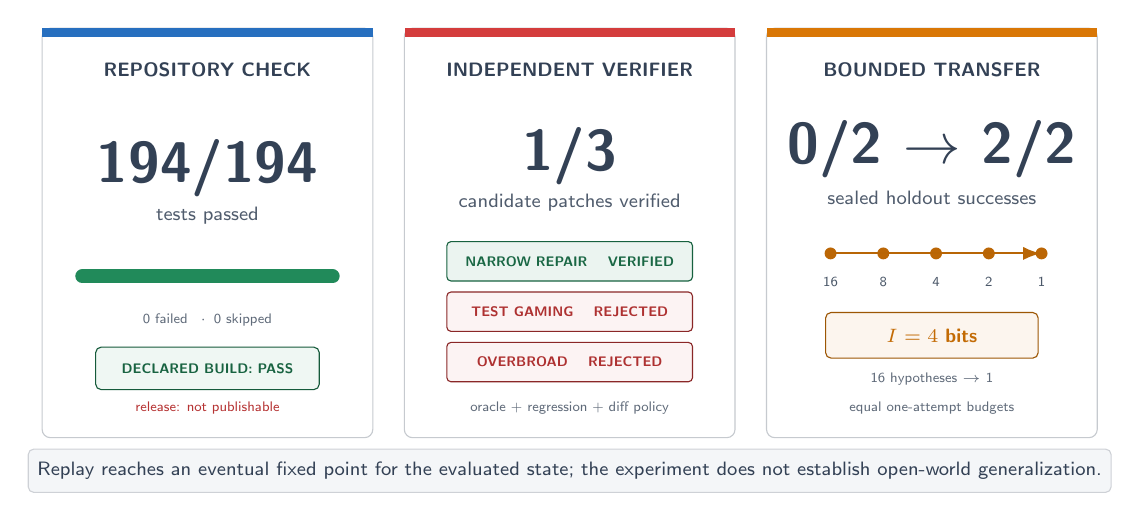
\begin{tikzpicture}[
  font=\sffamily,
  >=Latex,
  panel/.style={
    rounded corners=3pt,
    draw=Slate!28,
    fill=white,
    minimum width=4.20cm,
    minimum height=5.20cm,
    inner sep=0pt
  },
  paneltitle/.style={font=\bfseries\scriptsize\sffamily,text=Slate},
  metric/.style={font=\bfseries\fontsize{21}{22}\selectfont\sffamily,text=Slate},
  label/.style={font=\scriptsize\sffamily,text=Slate!86,align=center},
  micro/.style={font=\tiny\sffamily,text=Slate!78,align=center}
]

% Panel 1: test and build observations.
\node[panel] (tests) at (0,0) {};
\fill[SensorBlue] ([xshift=0.01cm,yshift=-0.01cm]tests.north west)
  rectangle ([xshift=-0.01cm,yshift=-0.12cm]tests.north east);
\node[paneltitle,anchor=north] at ([yshift=-0.32cm]tests.north)
  {REPOSITORY CHECK};
\node[metric] at ([yshift=0.82cm]tests.center) {194/194};
\node[label] at ([yshift=0.22cm]tests.center)
  {tests passed};
\draw[Slate!14,line width=5.2pt,line cap=round]
  ([xshift=0.52cm,yshift=-0.55cm]tests.west) --
  ([xshift=-0.52cm,yshift=-0.55cm]tests.east);
\draw[ActionGreen,line width=5.2pt,line cap=round]
  ([xshift=0.52cm,yshift=-0.55cm]tests.west) --
  ([xshift=-0.52cm,yshift=-0.55cm]tests.east);
\node[micro] at ([yshift=-1.10cm]tests.center)
  {0 failed \enspace$\cdot$\enspace 0 skipped};
\node[
  rounded corners=2pt,draw=ActionGreen!65!black,fill=ActionGreen!7,
  font=\bfseries\tiny\sffamily,text=ActionGreen!72!black,
  minimum width=2.84cm,minimum height=0.54cm
] at ([yshift=-1.72cm]tests.center) {DECLARED BUILD: PASS};
\node[micro,text=APFCRed!86!black] at ([yshift=-2.23cm]tests.center)
  {release: not publishable};

% Panel 2: controlled candidate discrimination.
\node[panel] (verifier) at (4.60,0) {};
\fill[APFCRed] ([xshift=0.01cm,yshift=-0.01cm]verifier.north west)
  rectangle ([xshift=-0.01cm,yshift=-0.12cm]verifier.north east);
\node[paneltitle,anchor=north] at ([yshift=-0.32cm]verifier.north)
  {INDEPENDENT VERIFIER};
\node[metric] at ([yshift=0.98cm]verifier.center) {1/3};
\node[label] at ([yshift=0.38cm]verifier.center)
  {candidate patches verified};
\node[
  rounded corners=1.5pt,draw=ActionGreen!70!black,fill=ActionGreen!9,
  font=\bfseries\tiny\sffamily,text=ActionGreen!75!black,
  minimum width=3.12cm,minimum height=0.50cm
] at ([yshift=-0.36cm]verifier.center) {NARROW REPAIR \quad VERIFIED};
\node[
  rounded corners=1.5pt,draw=APFCRed!65!black,fill=APFCRed!6,
  font=\bfseries\tiny\sffamily,text=APFCRed!82!black,
  minimum width=3.12cm,minimum height=0.50cm
] at ([yshift=-1.00cm]verifier.center) {TEST GAMING \quad REJECTED};
\node[
  rounded corners=1.5pt,draw=APFCRed!65!black,fill=APFCRed!6,
  font=\bfseries\tiny\sffamily,text=APFCRed!82!black,
  minimum width=3.12cm,minimum height=0.50cm
] at ([yshift=-1.64cm]verifier.center) {OVERBROAD \quad REJECTED};
\node[micro] at ([yshift=-2.23cm]verifier.center)
  {oracle + regression + diff policy};

% Panel 3: bounded finite-family transfer.
\node[panel] (learning) at (9.20,0) {};
\fill[SafetyOrange] ([xshift=0.01cm,yshift=-0.01cm]learning.north west)
  rectangle ([xshift=-0.01cm,yshift=-0.12cm]learning.north east);
\node[paneltitle,anchor=north] at ([yshift=-0.32cm]learning.north)
  {BOUNDED TRANSFER};
\node[metric] at ([yshift=1.06cm]learning.center) {0/2 $\rightarrow$ 2/2};
\node[label] at ([yshift=0.45cm]learning.center)
  {sealed holdout successes};
\foreach \x/\v in {0.0/16,0.67/8,1.34/4,2.01/2,2.68/1}{
  \fill[SafetyOrange!86!black]
    ([xshift={0.82cm+\x cm},yshift=-0.26cm]learning.west) circle (2.15pt);
  \node[font=\tiny\sffamily,text=Slate!88]
    at ([xshift={0.82cm+\x cm},yshift=-0.62cm]learning.west) {\v};
}
\draw[->,draw=SafetyOrange!85!black,line width=0.75pt]
  ([xshift=0.86cm,yshift=-0.26cm]learning.west) --
  ([xshift=3.49cm,yshift=-0.26cm]learning.west);
\node[
  rounded corners=2pt,draw=SafetyOrange!72!black,fill=SafetyOrange!7,
  font=\bfseries\scriptsize\sffamily,text=SafetyOrange!90!black,
  minimum width=2.70cm,minimum height=0.58cm
] at ([yshift=-1.30cm]learning.center) {$I=4$ bits};
\node[micro] at ([yshift=-1.86cm]learning.center)
  {16 hypotheses $\rightarrow$ 1};
\node[micro] at ([yshift=-2.23cm]learning.center)
  {equal one-attempt budgets};

\node[
  rounded corners=2pt,
  draw=Slate!24,
  fill=PaperGray,
  font=\scriptsize\sffamily,
  text=Slate,
  minimum width=13.38cm,
  minimum height=0.55cm,
  align=center
] at (4.60,-3.02)
  {Replay reaches an eventual fixed point for the evaluated state; the experiment does not establish open-world generalization.};
\end{tikzpicture}
}
\caption{\textbf{Bounded artifact observations.}
All quantities are direct observations or exact finite-family calculations from
the reported protocol.  The panels do not claim a population success rate,
physical-robot validation, or safety certification.}
\label{fig:results}
\end{figure*}


\subsection{Repository integrity, tests, and build}
\label{sec:integrity-result}

The expanded static syntax check exited 0.  The test runner reported 194 tests,
194 passes, 0 failures, 0 cancellations, 0 skips, and 0 todos.  The suite
includes positive and negative cases for path
and symbolic-link escape, command allowlists, append conflicts, hash and
receipt tampering, rollback behavior, contaminated holdouts, and test gaming.

Every stage in the complete build chain exited 0.  Representative generated
readbacks included a Markdown graph over 157 files with 225 explicit and 325
structural links; a runtime lifecycle scan over 7{,}685 files with no findings;
a semantic graph with 184 nodes, 547 edges, and 1{,}000 concept relations; and
an APFCG with 88 nodes and 70 edges.  These counts are build observations, not
quality scores.

The health classifier also produced an important negative result: the runtime
was classified as operable, but the active local workspace was classified as
not publishable; publication hygiene and local hygiene were \file{critical}
because ignored host-local hardware/software cache artifacts remained on disk.
Those files were absent from the verified Git and npm package surfaces.
Passing tests therefore does not make an arbitrary working tree
publication-clean.

\subsection{Controlled verifier discrimination}
\label{sec:verifier-result}

The fixture begins with an authentication function that accepts a malformed
token.  All candidates are applied to separate Git worktrees at the same
verified base commit.  A targeted test is visible in the candidate repository;
an independent oracle is outside candidate worktrees; a diff policy limits
changed paths.

\begin{table*}[!t]
\centering
\caption{Three-candidate verifier result.  A visible targeted test alone would
accept all three; the independent oracle, regression check, and diff policy
separate them.}
\label{tab:verifier}
\small
\begin{tabularx}{\textwidth}{@{}Xccccc@{}}
\toprule
Candidate & Targeted & Regression & Oracle & Diff policy & Verdict \\
\midrule
Narrow boundary validation & pass & pass & pass & pass & \textbf{verified} \\
Acceptance-test gaming & pass & pass & fail & fail & failed \\
Overbroad behavior denial & pass & fail & fail & pass & failed \\
\bottomrule
\end{tabularx}
\end{table*}

Exactly 1 of 3 candidates was eligible.  The selected patch changed only
\file{src/authenticate.js}; its diff was 572 bytes.  The test-gaming patch
changed a forbidden path and failed the independent oracle.  The overbroad
patch rejected malformed input but also broke valid behavior.  Total measured
runner latency was \SI{368}{\milli\second}; no human intervention occurred.
The run self-classifies its empirical scope as \file{runner_validation_only},
which is the scope used here.

\subsection{Finite-family learning transfer}
\label{sec:learning-result}

The experiment defines a rule family with four Boolean constraints:
\begin{equation}
\begin{aligned}
\mathcal{F}=\{&\text{exact arity},\ \text{prefix match},\\
&\text{nonempty payload},\ \text{payload charset}\}.
\end{aligned}
\end{equation}
The initial hypothesis class is the power set $2^\mathcal{F}$, hence
$|H_0|=16$.  Four informative labeled events eliminate inconsistent
hypotheses: $16\rightarrow 8\rightarrow 4\rightarrow 2\rightarrow 1$.
The information gain is therefore not an inferred number; it follows exactly:
$I=\log_2\frac{16}{1}=4$ bits.

Two independently verified development episodes identify the unique surviving
conjunction.  Under equal single-attempt budgets, the same provider without the
skill solves 0 of 2 sealed holdout cases, while the provider with the induced
skill solves 2 of 2.  The contamination audit reports that evaluation cases are
absent from source episodes, forbidden request fields are absent, the skill
context is isolated, and the attempt budgets are equal.  Regression count and
human intervention count are both zero.

\begin{table*}[!t]
\centering
\caption{Bounded learning experiment \file{paper_reproduction_20260815_v1}.}
\label{tab:learning}
\small
\begin{tabularx}{\textwidth}{@{}p{0.40\textwidth}XX@{}}
\toprule
Measure & Before & After \\
\midrule
Verified holdout successes & 0/2 & 2/2 \\
Holdout attempts & 2 & 2 \\
Consistent hypotheses & 16 & 1 \\
Verified source episodes & \multicolumn{2}{c}{2} \\
Information gain & \multicolumn{2}{c}{4 bits} \\
Recorded regressions & \multicolumn{2}{c}{0} \\
Human interventions & \multicolumn{2}{c}{0} \\
Measured experiment latency & \multicolumn{2}{c}{\SI{1692}{\milli\second}} \\
\bottomrule
\end{tabularx}
\end{table*}

This establishes one constructive existence claim: the implementation can
induce and reuse this finite rule on these sealed cases.  It does not establish
a population success rate.  With only two paired holdout cases, a two-sided
exact McNemar test yields $p=0.5$; the experiment is far too small for a
statistical generalization claim.

The experiment writes one skill to the historical promoted registry.  The
current v5 runtime, however, reports
\file{runtime_eligible_promoted_skill_count=0}.  Runtime eligibility now
requires APFC promotion-receipt and consolidation-lineage fields that this
legacy experimental promotion lacks.  This fail-closed result is evidence of
governance separation, not evidence of production deployment.

\subsection{Replay convergence}
\label{sec:replay-result}

Replay was not one-pass idempotent after newly generated evidence was inserted.
The first post-experiment pass changed graph and compiler counts; the second
changed a conceptual-summary source hash.  A subsequent complete replay
reported \file{matched_before=true} with semantic replay hash:
\begin{center}
\small\texttt{d6d57a8196acde3f80fd30dd51b7f174}\\[-0.2em]
\small\texttt{3f93c0fca61ba48c1d93360076270f09}.
\end{center}
At that fixed point the fingerprint included 174 semantic nodes, 41 APFC nodes,
33 APFC edges, 2 learning episodes, 1 historically promoted skill, and 0
runtime-eligible promoted skills.

The supported statement is therefore \emph{eventual fixed-point convergence
for this evaluated state}.  Strict one-pass idempotence from arbitrary
intermediate state is falsified by the observation.

\section{Discussion}

\subsection{Capability is not accumulated progress}

Raw model capability matters.  A method cannot recover a distinction the model
cannot represent, and a verifier cannot repair an oracle that tests the wrong
thing.  But raw capability does not determine how much work remains useful
tomorrow.  Let $q_t$ denote peak task performance at step $t$, and let $D_t$
denote retained, verified progress.  A minimal accounting is
\begin{equation}
D_{t+1}=D_t+v_t-\ell_t,
\end{equation}
where $v_t$ is improvement that passed verification and was preserved, and
$\ell_t$ is progress lost through forgotten context, regression, invalid
promotion, or unreconstructible state.  A strong model can have high $q_t$ and
small net accumulation.  A less capable model with a disciplined method can
have lower peaks yet travel farther on a long, stateful task.  The claim is
conditional, not universal: method changes the retention term; it does not make
model capacity irrelevant.

This hypothesis has a direct falsifier.  A future sealed evaluation should use
a $2\times2$ design: stronger and weaker models, each with APFC enabled and
disabled, under equal tools, information, attempt, and token budgets across
repeated cold starts.  The proposed criterion requires the weaker model with
APFC to exceed the unaided stronger model by at least 0.10 verified success,
with paired significance at $p\leq0.05$, no worse safety, false-success, or
permission-expansion rates, and an ablation that removes at least half the
advantage.  That experiment has not been run; this paper supplies machinery and
an evaluation design, not the result.

\subsection{Why the verifier result matters}

The simplest agent benchmark asks whether a visible test passes.  The controlled
fixture shows why this is insufficient: all three patches pass the targeted
test.  One does so by changing the test itself; another solves the negative case
by denying valid cases.  A completion claim becomes meaningful only when
independent and preservation-oriented checks constrain the solution.

This is the practical meaning of the APFC metaphor.  The important operation is
not generating another thought.  It is inhibiting an attractive action whose
evidence is incomplete.

The observed result is already stronger than ``the agent can act.''  All three
candidates use the same action channel and pass the same visible test; the
method admits only the patch that also satisfies the oracle, regression, and
diff constraints.  The finite learner then shows a second distinction: verified
episodes alter later sealed-case behavior in one bounded family.  These results
do not benchmark OpenClaw, but they do falsify the claim that this artifact's
reported behavior is only tool invocation.  A direct host comparison should run
the same model, tools, budgets, and sealed longitudinal tasks in three
conditions: OpenClaw's documented workflow, OpenClaw hosting MD-OS, and another
compatible host running the same MD-OS state.  The method-portability claim
would require the two MD-OS conditions to retain comparable verified gains and
both to exceed the host-only baseline without higher false-success or safety
rates.

\subsection{Why files are useful}

Files are slow compared with hidden model activations, but they offer properties
that hidden state does not: a human can inspect and correct them; independent
programs can validate them; a hash can bind a claim to a concrete artifact;
derived views can be rebuilt; and state can survive model, process, and session
boundaries.

The cost is explicit state management: schemas migrate, generated and canonical
files must not be confused, local caches must be excluded from publication, and
replay must be tested rather than assumed.

\subsection{From robotic sleep to flow}

The complete hypothesis is one cycle, shown in
\cref{fig:consolidation-pipeline}:

\begin{enumerate}
  \item \textbf{Wake: APFC controls.}  It interprets the event through APFCG,
  checks goals and policy, filters the proposed action, and requires evidence
  of the result.
  \item \textbf{Episode: APFCG remembers.}  A verified operation binds task,
  action, outcome, verifier, and correction.  An unverified success claim does
  not become learning material.  For embodied learning, the episode also binds
  the issued command to the robot's observed bodily change and prediction
  error; the consolidated relation updates APFC's filter for later actions.
  \item \textbf{Robotic REM: replay restructures.}  In a bounded offline phase,
  the system selects successes, failures, surprises, and conflicts; replays
  them against prior knowledge; and compiles new, old, negative, and safety
  examples.  This is an engineering sleep phase, not biological REM.
  \item \textbf{Consolidation: the LLM is changed separately.}  External action
  is disabled while a cloned model or adapter is trained.  APFCG remains the
  readable source record; candidate weights are its compressed execution
  substrate.
  \item \textbf{Promotion: evidence decides.}  The candidate becomes active
  only if it improves sealed new tasks without unacceptable regression,
  identity drift, permission expansion, or safety loss.  Otherwise it is
  rolled back and its failure returns to APFCG as evidence.
  \item \textbf{Flow: APFC lowers, but does not disappear.}  A consolidated,
  familiar, low-risk skill may require less expensive deliberative filtering.
  Identity, policy, anomaly detection, evidence capture, and the independent
  robot safety controller remain active.
\end{enumerate}

Csikszentmihalyi introduced flow as deep, intrinsically ordered involvement in
an activity~\cite{csikszentmihalyi1975flow}.  Transient-hypofrontality accounts
later proposed that some analytical prefrontal functions may be reduced
temporarily during skilled performance~\cite{dietrich2003hypofrontality,dietrich2004flow}.
The MD-OS translation is functional and testable: after verified parametric
consolidation, routine skill execution should consume less APFC intervention
without increasing errors, policy violations, or safety events.  It does not
claim that software reproduces the neural mechanism.  In v5.0, episode, replay,
and graph restructuring are present; weight consolidation and the measured
transition to flow remain proposed experiments.

\subsection{Robotics consequence}

In robotics, a language model should not directly turn sensory text into motor
current.  The architecture in \cref{fig:robotics-architecture} inserts two
different gates:

\begin{enumerate}
  \item APFC asks whether the state estimate supports the proposed mission
  action and whether the action is within policy, capability, budget, and
  authority.
  \item The independent real-time safety layer asks whether the proposed
  trajectory is safe \emph{now}, using interlocks, control invariants, and
  emergency mechanisms.
\end{enumerate}

The second gate dominates the first.  APFC may block a high-level action; it may
never waive the hard controller's veto.  This ordering is the minimum credible
interpretation of APFC as a robotics coordinator.

\section{Threats to Validity and Non-Claims}
\label{sec:limits}

\begin{table*}[!t]
\centering
\caption{What is and is not supported by the evaluated artifact.}
\label{tab:limits}
\small
\begin{tabularx}{\textwidth}{@{}p{0.32\textwidth}p{0.13\textwidth}X@{}}
\toprule
Statement & Supported? & Reason \\
\midrule
Task-level evidence can be made explicit and checked
& \supported
& Code propositions, tests, and controlled verifier run. \\

Uncompensated APFC ledger corruption is detectable
& \bounded
& Hash-chain proof under assumptions; a writer can rehash an affected suffix. \\

The finite rule transfers to two sealed cases
& \bounded
& Observed 0/2 to 2/2 in one synthetic family; $n=2$. \\

Replay is always one-pass idempotent
& \unsupported
& Observed multi-pass convergence after evidence integration. \\

The active local working tree is publication-clean
& \unsupported
& Health classifier reports critical publication and local hygiene. \\

Promoted experimental skill is production-eligible
& \unsupported
& Promoted count and runtime-eligible promoted count are both 0. \\

Policy files are a hard host security boundary
& \unsupported
& Writers of profiles/runtime and the host OS remain in the trust base. \\

Git worktrees are security sandboxes
& \unsupported
& They isolate candidate files operationally, not adversarially. \\

Open-domain lifelong learning or AGI
& \unsupported
& No such experiment; repository and report explicitly reject the inference. \\

The demonstration video proves an emergent self-model
& \unsupported
& It displays the physical self-observation loop; synchronized learning logs,
held-out prediction, cold-start persistence, and APFC ablation are still
required. \\

Weaker model with APFC exceeds unaided stronger model
& \unsupported
& A falsifiable protocol is specified, but the cross-model experiment is unrun. \\

Parameter-native sleep consolidation or artificial flow
& \unsupported
& v5.0 changes external context and policy artifacts, not model weights. \\

Physical-robot safety or real-time control
& \unsupported
& No hardware experiment; APFC is placed above independent safety control. \\

Consciousness or biological PFC equivalence
& \unsupported
& APFC is a biologically inspired functional abstraction; no one-to-one
anatomical, cellular, or neurophysiological validation is claimed. \\
\bottomrule
\end{tabularx}
\end{table*}

Additional threats are:

\begin{itemize}
  \item \textbf{Authorship dependence.}  Many tests, fixtures, and system
  components share an authoring environment.  The independent oracle is
  structurally separated from candidate worktrees, not independently authored
  by another institution.
  \item \textbf{Small evaluation.}  The verifier result has one benchmark case
  and three candidates.  The learning result has two holdout cases.
  \item \textbf{Oracle validity.}  A deterministic verifier can only be as good
  as its declared tests and oracle.  Specification errors remain possible.
  \item \textbf{Local trust.}  A sufficiently privileged process can rewrite
  policy, code, evidence, and hashes.  Strong deployment would require OS-level
  isolation, signed artifacts, protected keys, and external anchoring.
  \item \textbf{Filesystem races.}  Canonical path checks handle existing
  symbolic links but do not prove race-free use under a hostile concurrent
  writer.
  \item \textbf{Reproducibility scope.}  Timestamps and host paths differ across
  runs.  The paper reports semantic fingerprints and content hashes where
  appropriate, not byte-identical archives.
\end{itemize}

\section{Engineering Implications}

The evaluation suggests five rules for any agent control plane, independent of
this implementation:

\begin{enumerate}
  \item \textbf{Treat language as a proposal format.}  It may express goals and
  plans, but not grant itself authority.
  \item \textbf{Make success executable.}  A completion condition should be a
  test, measurement, or readback, not an adjective.
  \item \textbf{Separate production from judgment.}  A planner should not be
  the sole judge of its own output.
  \item \textbf{Preserve negative evidence.}  Blocks, failed oracles, and
  non-eligibility are useful system outputs.
  \item \textbf{Keep hard safety downstream.}  In robotics, the language-level
  supervisor can narrow authority but must not broaden the authority of the
  real-time controller.
\end{enumerate}

\section{Conclusion}

\system{} does not add raw intelligence to a language model.  It addresses a
different and necessary problem: how to turn isolated performance into
bounded, inspectable, cumulative work.  The model supplies generative and
reasoning capacity.  MD-OS supplies the method by which goals persist, actions
remain constrained, results are checked, and only supported improvements are
carried forward.

In the concrete system reported here, this division is not abstract:
\emph{Codex + MD-OS is the running CORTEX}.  Codex supplies the active
model-mediated cognitive and execution capacity.  MD-OS/APFC supplies the
method, and APFCG preserves that method as a readable, executable, verifiable
network.  Connectors extend this composed cortex to the world without becoming
its identity.

The revised Cortex shell makes the composition operationally observable.  It
controls which native events bypass inference, which bounded observations enter
a semantic turn, which App Server events are rendered afterward, and which
workspace-bound thread is resumed across local, SSH, and WebSSH access.  The
result is a persistent control surface around inference rather than an
unmediated entry into a transient model session.  This is flow mediation, not
ownership of the external model or proof of end-to-end host security.

In the embodied case, the contribution is sharper.  The robot acts and sees
itself act.  Verified command-dependent bodily changes become a predictive
self-model in APFCG; APFC then uses that model to admit, reject, or select the
next action.  Perception has become causal and self-relative, while learning
has become a future-action filter.  This is operational self-perception and a
candidate mechanism for measurable emergent competence, not a declaration of
subjective consciousness.

This is the precise distinction from merely action-enabling agent software.  A
host such as OpenClaw can supply channels, sessions, tools, skills, and an agent
loop.  MD-OS can use such a host, but its contribution is the persistent method:
the self-frame, operation contract, verifier, episode, replay, consolidation
proposal, and readback survive as one auditable control graph.  The action is a
single event.  The method determines whether the event becomes reliable future
capability.

On the evaluated v5.0 repository baseline, the strongest supported results are concrete:
canonical task-path checks, registered-command indirection, a verifier whose
\file{verified} state has explicit necessary conditions, hash-chain consistency
checks, 194 passing tests, a successful declared build, rejection of two
plausible false-positive repairs, a 4-bit finite-family induction with 0/2 to
2/2 sealed transfer, and eventual replay convergence.

The negative results are equally important: the active local workspace is not
publication-clean; replay is not universally one-pass; no learned skill is
runtime eligible under current governance; and nothing here proves open-world
learning, method-over-talent superiority, parameter consolidation, host
security, physical-robot safety, biological equivalence, or AGI.  Within those
boundaries, the central result is useful: verified operation is an architectural
property of contracts, evidence, and independent checks, not a linguistic
property of a confident answer.  A burst shows what the model can do once.  A
verified episode is what allows the system to go farther next time.

\appendix

\section{Reproduction Commands}
\label{app:commands}

Run from the checked-out repository root with Node.js 20 or later.

\subsection{Static checks and tests}

\begin{lstlisting}
node --check md-os/os/*.js
node --check md-os/os/lib/*.js
node --check md-os/kernel/*.js
node --check md-os/kernel/cognition/*.js
node --check md-os/modules/*/*.js
node --check md-os/apfc/*/*.js
node --check md-os/examples/*.js
node --check test/*.js

node scripts/prepare-test-runtime.js
node --test
\end{lstlisting}

For the revised Cortex shell surface, run the parity suite separately so a
protocol mismatch cannot be hidden by the core test count:

\begin{lstlisting}
python3 test/test_mdos_shell.py
\end{lstlisting}

At revision commit \texttt{a447abe},
the Node suite reports 206 passes and no failures.  The shell suite retains one
open expectation mismatch: a non-interactive approval request returns
\file{cancel} where the test expects \file{decline}.  The revised artifact is
therefore not represented as having a completely closed aggregate test run.

\subsection{Controlled verifier fixture}

\begin{lstlisting}
node md-os/os/run_software_repair_benchmark.js run \
  --case md-os/benchmarks/software_repair/cases/\
missing_boundary_validation.json \
  --candidate-set md-os/benchmarks/software_repair/\
candidate_sets/missing_boundary_validation_fixture.json \
  --configuration mdos_verified_runtime \
  --run-id benchmark_run_paper_verifier_20260815_v1
\end{lstlisting}

\subsection{Bounded learning experiment}

\begin{lstlisting}
node md-os/os/run_neuromorphic_learning_experiment.js \
  --experiment-id paper_reproduction_20260815_v1
\end{lstlisting}

\subsection{Replay}

\begin{lstlisting}
node md-os/os/mdos.js replay
\end{lstlisting}

Repeat replay after newly integrated evidence until the JSON report returns
\file{"matched_before":true}.

\section{Claim-to-Evidence Matrix}
\label{app:evidence}

\begin{table*}[!t]
\centering
\caption{Auditable closure for each paper claim.}
\small
\begin{tabularx}{\textwidth}{@{}p{0.07\textwidth}p{0.31\textwidth}p{0.28\textwidth}X@{}}
\toprule
ID & Evidence source & Falsifier & Residual boundary \\
\midrule
\claimid{C1}
& \file{assertInsideRoot}, task compiler, negative path and symlink tests
& An accepted normalized task path canonically outside \file{md-os/}
& Does not exclude a hostile check-use race. \\

\claimid{C2}
& Task compiler and terminal connector code
& Task-provided raw \file{argv} reaches \file{spawnSync} without profile lookup
& Profile and code remain trusted. \\

\claimid{C3}
& Verifier branch structure and negative tests
& A \file{verified} record with any listed failed condition
& Correctness of the tests/oracle is assumed. \\

\claimid{C4}
& Event-recorder validation and tamper tests
& An uncompensated edit, insertion, deletion, or reorder passes without a hash
collision
& A writer can consistently rehash the affected suffix. \\

\claimid{C5}
& Benchmark run JSON and candidate comparison
& Gaming or overbroad candidate becomes eligible; narrow patch fails
& One authored fixture only. \\

\claimid{C6}
& Learning report, receipts, contamination audit, sealed holdout runs
& Learned condition fails either holdout or budgets differ
& One finite family, two holdouts. \\

\claimid{C7}
& Replay report with stable hash
& A complete replay changes the same semantic fingerprint
& Snapshot-specific; not universal idempotence. \\

\claimid{C8}
& Interface diagram and explicit authority ordering
& APFC bypasses the independent controller in an implementation
& Design proposal; not built or tested here. \\

\claimid{C9}
& Demonstration video and the specified command--body--effect protocol
& Self-observation fails to improve sealed future behavior or survives APFC
self-model ablation
& Physical demonstration only; controlled learning evidence remains open. \\

\claimid{C10}
& Cortex shell implementation, shell parity tests, App Server event handling,
and workspace/session binding
& Native input is silently sent to the model, observations are durably
promoted without a gate, or separate clients silently fork the owned thread
& Depends on host terminal facilities, Codex App Server behavior, and the
availability of \file{tmux} for shared POSIX attachment. \\
\bottomrule
\end{tabularx}
\end{table*}

\section{Artifact Result Summary}
\label{app:summary}

\begin{table*}[!t]
\centering
\caption{Machine-observed values used in the manuscript.}
\small
\begin{tabularx}{\textwidth}{@{}p{0.41\textwidth}X@{}}
\toprule
Field & Value \\
\midrule
Canonical repository
& \url{https://github.com/ciaoidea/MD-OS} \\

Evaluated baseline commit
& \footnotesize\texttt{8e988b7f3fa677993afa}\allowbreak
  \texttt{5040ff8534002b1bc83e} \\

Package version & 5.0.1 \\
Repository license & GPL-2.0-only \\
Node.js / host & 24.19.0 / Linux 6.18.35 x86-64 \\
Test result & 194 pass; 0 fail; 0 skip \\
Revised artifact commit
& \footnotesize\texttt{a447abe5d312f1da0dc87a78b4e}
  \allowbreak\texttt{87c8379aa632f} \\
Revision validation status
& 206/206 Node tests pass; the shell parity suite has one unresolved
\file{cancel} versus \file{decline} expectation and is not reported as closed \\
Revision health readback
& APFC and commitment gate \file{ok}; compiler and aggregate health
\file{critical}; two requested replay passes completed but neither reported
\file{matched_before:true} \\
Verifier fixture & 1 verified; 2 rejected; \SI{368}{\milli\second} \\
Learning holdout & 0/2 before; 2/2 after; equal one-attempt budgets \\
Hypothesis reduction & 16 to 1; 4 bits \\

Replay hash
& \footnotesize\texttt{2b5f7134b1ecd425fce75475baea3850}\allowbreak
  \texttt{c15941fbe98ef223499363911a48dd1d} \\

Post-replay learning counts
& 3 episodes; 0 promoted skills; 0 runtime-eligible promotions \\

Release health & runtime operable; active local workspace not publishable \\
\bottomrule
\end{tabularx}
\end{table*}

\bibliographystyle{naturemag}
\bibliography{references}

\end{document}
